% Modelo de TCC do Bacharelado em Ciência da Computação da UNIFESP 
% Baseado no Modelo de Documentos Academicos do ABNTex2  

\documentclass[	12pt, Times, openright, twoside, a4paper, english, brazil]{abntex2}

% ---
% Pacotes fundamentais 
% ---
\usepackage{cmap}				% Mapear caracteres especiais no PDF
%\usepackage{lmodern}			% Usa a fonte Latin Modern			
\usepackage{times}
\usepackage[T1]{fontenc}			% Selecao de codigos de fonte.
\usepackage[utf8]{inputenc}		% Codificacao do documento (conversão automática dos acentos)
\usepackage{lastpage}			% Usado pela Ficha catalográfica
%\usepackage{natbib}
\usepackage{indentfirst}			% Indenta o primeiro parágrafo de cada seção.
\usepackage{color}				% Controle das cores
\usepackage{graphicx}			% Inclusão de gráficos
\usepackage{tikz}
\usepackage{array} 

\def\checkmark{\tikz\fill[scale=0.4](0,.35) -- (.25,0) -- (1,.7) -- (.25,.15) -- cycle;} 
\newcolumntype{L}[1]{>{\raggedright\let\newline\\\arraybackslash\hspace{0pt}}m{#1}}
\newcolumntype{C}[1]{>{\centering\let\newline\\\arraybackslash\hspace{0pt}}m{#1}}
\newcolumntype{R}[1]{>{\raggedleft\let\newline\\\arraybackslash\hspace{0pt}}m{#1}}
% ---


% ---
% Pacotes de citações
% ---
\usepackage[brazilian,hyperpageref]{backref}	 % Paginas com as citações na bibl
\usepackage[alf]{abntex2cite}	% Citações padrão ABNT

% --- 
% CONFIGURAÇÕES DE PACOTES
% --- 

% ---
% Configurações do pacote backref
% Usado sem a opção hyperpageref de backref
\renewcommand{\backrefpagesname}{Citado na(s) página(s):~}
% Texto padrão antes do número das páginas
\renewcommand{\backref}{}
% Define os textos da citação
\renewcommand*{\backrefalt}[4]{
	\ifcase #1 %
		Nenhuma citação no texto.%
	\or
		Citado na página #2.%
	\else
		Citado #1 vezes nas páginas #2.%
	\fi}%
% ---

% numeração de figuras e tabelas 
\counterwithout{figure}{section}
\counterwithout{table}{section}

%\renewcommand\tablename{Tabela{\arabic{chapter}.}}


% ---
% Informações de dados para CAPA e FOLHA DE ROSTO
% ---
\titulo{Ferramenta para auxiliar daltônicos a distinguir cores}
\autor{Paulo Sérgio de Souza Neves}
\local{São José dos Campos, SP}
\data{Novembro de 2014}
\orientador{Profa. Dra. Ana Luísa Dine Martins Lemos}

%\coorientador{Prof. Dr. Beltrano da Silva}
\instituicao{%
  Universidade Federal de São Paulo -- UNIFESP
  \par
  Instituto de Ciência de Tecnologia
  \par
  Bacharelado em Ciência da Computação}
\tipotrabalho{Trabalho de Graduação}
% O preambulo deve conter o tipo do trabalho, o objetivo, 
% o nome da instituição e a área de concentração 
\preambulo{Trabalho de conclusão de curso apresentado ao Instituto de Ciência e Tecnologia – UNIFESP, como parte das atividades para obtenção do título de Bacharel em Ciência da Computação.}
% ---

% informações do PDF
\makeatletter
\hypersetup{
     	%pagebackref=true,
		pdftitle={\@title}, 
		pdfauthor={\@author},
    	pdfsubject={\imprimirpreambulo},
	    pdfcreator={LaTeX with abnTeX2},
		pdfkeywords={abnt}{latex}{abntex}{abntex2}{trabalho acadêmico}, 
		colorlinks=true,       		% false: boxed links; true: colored links
    	linkcolor=blue,          	% color of internal links
    	citecolor=blue,        		% color of links to bibliography
    	filecolor=magenta,      	% color of file links
		urlcolor=blue,
		bookmarksdepth=4
}

\makeatother
% --- 
% --- 
% Espaçamentos entre linhas e parágrafos 
% --- 
% O tamanho do parágrafo é dado por:
\setlength{\parindent}{1.3cm}
% Controle do espaçamento entre um parágrafo e outro:
\setlength{\parskip}{0.2cm}  % tente também \onelineskip
% ---

% compila o indice
% ---
\makeindex
% ---

% ----
% Início do documento
% ----
\begin{document}
% Retira espaço extra obsoleto entre as frases.
\frenchspacing 

% ----------------------------------------------------------
% ELEMENTOS PRÉ-TEXTUAIS
% ----------------------------------------------------------
% \pretextual

% ---
% Capa
% ---
\begin{capa}
  \begin{center}
   
\includegraphics[width=.25\textwidth]{logo-unifesp.pdf}
    \vspace*{\fill}
    
    {\ABNTEXchapterfont\large\imprimirautor}
    \vspace*{\fill}
    
    {\ABNTEXchapterfont\bfseries\Large\imprimirtitulo}
    \vspace*{\fill}\vspace*{\fill}
    
   \imprimirlocal
   \end{center}
\end{capa}

% ---
% Folha de rosto
% (o * indica que haverá a ficha bibliográfica)
% ---
\imprimirfolhaderosto*
% ---

% ---
% Inserir folha de aprovação
% ---
% Isto é um exemplo de Folha de aprovação, elemento obrigatório da NBR
% 14724/2011 (seção 4.2.1.3). Você pode utilizar este modelo até a aprovação
% do trabalho. Após isso, substitua todo o conteúdo deste arquivo por uma
% imagem da página assinada pela banca com o comando abaixo:
%
% \includepdf{folhadeaprovacao_final.pdf}
%
\begin{folhadeaprovacao}
  \begin{center}
    {\ABNTEXchapterfont\large\imprimirautor}

    \vspace*{\fill}\vspace*{\fill}
    {\ABNTEXchapterfont\bfseries\Large\imprimirtitulo}
    \vspace*{\fill}
    
    \hspace{.45\textwidth}
    \begin{minipage}{.5\textwidth}
        \imprimirpreambulo
    \end{minipage}%
    \vspace*{\fill}
   \end{center}
    
   Trabalho aprovado em 02 de Dezembro de 2014:

   \assinatura{\textbf{\imprimirorientador} \\ Orientador} 
   \assinatura{\textbf{Professor} \\ Convidado 1}
   \assinatura{\textbf{Professor} \\ Convidado 2}
   \assinatura{\textbf{Professor} \\ Convidado 3}
   %\assinatura{\textbf{Professor} \\ Convidado 4}
      
   \begin{center}
    \vspace*{0.5cm}
    {\large\imprimirlocal}
    \par
    {\large\imprimirdata}
    \vspace*{1cm}
  \end{center}
  
\end{folhadeaprovacao}
% ---

% ---
% Dedicatória
% ---
\begin{dedicatoria}
   \vspace*{\fill}
   \centering
   \noindent
   \textit{Dedico este trabalho aos meus pais e avós.} \vspace*{\fill}
\end{dedicatoria}
% ---

% ---
% Agradecimentos
% ---
\begin{agradecimentos}
Agradeço aos meus pais César de Paula Neves e Rosa Lina de Souza Neves por me darem estrutura para que fosse possível completar meus objetivos, aos meus avós que me acolheram em São José dos Campos para estudar no Instituto de Ciência de Tecnologia da Universidade Federal de São Paulo e a todos os demais familiares e amigos que incentivaram meus estudos.


\end{agradecimentos}
% ---

% ---
% Epígrafe
% ---
\begin{epigrafe}
    \vspace*{\fill}
	\begin{flushright}
		\textit{"Controle a sua mente ou ela o controlará."}
	\end{flushright}
\end{epigrafe}
% ---

% ---
% RESUMOS
% ---

% resumo em português
\begin{resumo}
O daltonismo é uma deficiência que atinge cerca de 8\% da população masculina mundial. Raros são os casos de daltonismo em que as pessoas enxergam apenas tons de cinza, a maioria dos daltônicos enxergam as cores mas possuem dificuldade em distingui-las. Essa dificuldade de diferenciar as cores causa problemas em atividades cotidianas de pessoas portadoras de daltonismo. Com a finalidade de minimizar esses problemas, este trabalho tem como objetivo apresentar uma ferramenta para auxiliar daltônicos a diferenciarem cores.

 \vspace{\onelineskip}
    
 \noindent
 \textbf{Palavras-chaves}: Daltonismo. Processamento de imagens. 
\end{resumo}

\begin{resumo}[Abstract]
 \begin{otherlanguage*}{english}
Color blindness is a disability that affects about 8\% of the world male population. The color blindness cases which people see only shades of gray are rare, most color blinds see colors but they have difficulty in distinguishing them. This difficulty of differentiating the colors cause problems in everyday activities of people suffering from color blindness. For try to minimize these problems, this manual proposes the creation of a tool, which will process images for help color blinds to differentiate colors.

\vspace{\onelineskip}
 
   \noindent 
   \textbf{Key-words}: Color blind. Imagem processing.
 \end{otherlanguage*}
\end{resumo}

% ---
% inserir lista de figuras
% ---
\pdfbookmark[0]{\listfigurename}{lof}
\listoffigures*
\cleardoublepage
% ---

% ---
% inserir lista de tabelas
% ---
\pdfbookmark[0]{\listtablename}{lot}
\listoftables*
\cleardoublepage
% ---

% ---
% ---

\begin{siglas}
  \item[API] Application Programming Interface
  \item[CMY] Cyan, Magenta and Yellow
  \item[HSB] Hue, Saturation and Brightness
  \item[HSI] Hue, Saturation and Intensity
  \item[HSV] Hue, Saturation and Value
  \item[LMS] Longwave, Middlewave and Shortwave
  \item[PaaS] Platform as a Service
  \item[RGB] Red, Green and Blue
  \item[TCC] Trabalho de Conclusão de Curso
  

\end{siglas}
% ---

% ---
% inserir lista de símbolos
% ---
\begin{simbolos}
  \item[$ \delta $] Letra grega Delta
\end{simbolos}
% ---

% ---
% inserir o sumario
% ---
\pdfbookmark[0]{\contentsname}{toc}
\tableofcontents*
\cleardoublepage
% ---

% ----------------------------------------------------------
% ELEMENTOS TEXTUAIS
% ----------------------------------------------------------
\textual

% ----------------------------------------------------------
% Introdução
% ----------------------------------------------------------
\chapter{Introdução}

A retina é uma membrana que está localizada dentro de nossos olhos. Dentro da retina existem receptores que podem ser classificados em duas categorias: os bastonetes (cerca de 120 milhões) e cones (cerca de 6 milhões) \cite{koschan2008}. Existem três tipos de cones, os que identificam ondas curtas (S), médias (M) e longas (L). Os cones do tipo S são sensíveis à luz azul, os cones do tipo M são sensíveis a luz verde e os cones do tipo L são sensíveis a cor vermelha. Dos cones existentes no sistema visual dos seres humanos, cerca de 65\% são sensíveis a luz vermelha, 33\% a luz verde e 2\% são sensíveis a luz azul, e os cones sensíveis a luz azul são os mais sensíveis \cite{gonzalez2008}. Com a mistura da intensidade capturada por cada tipo de cone é possível realizar combinações que permitem ao olho humano identificar milhões de cores.

A maioria dos daltônicos são pessoas com dificuldade de diferenciar cores por causa da deficiência total ou parcial de 1, 2 ou 3 tipos de cones. A deficiência total de um tipo de cone é definida pela sua total ausência na retina. Apenas daltônicos com deficiência total em dois ou três tipos de cones não conseguem identificar cor alguma. No entanto, essa deficiência é extremamente rara e atinge menos de 1\% dos daltônicos.

A deficiência do daltonismo é carregada pelo cromossomo X. Os homens possuem apenas um cromossomo X e as mulheres possuem dois. Uma mulher será daltônica apenas se os dois cromossomos X forem deficientes e por esse motivo existem muitos mais homens daltônicos do que mulheres. Cerca de 7 a 10\% dos homens são daltônicos, enquanto menos de 1\% das mulheres possuem essa deficiência \cite{mcdowell2008}. Excepcionalmente, o daltonismo pode não ser herdado dos pais, sendo causado por algum acidente envolvendo os olhos, cérebro ou nervos.

Uma imagem digital colorida pode ser representada por uma função $f(x, y)$ onde $x$ e $y$ são as coordenadas espaciais de um plano de duas dimensões. Se o sistema de cores utilizado for o sistema RGB, que será apresentado posteriormente, $f(x, y)$ é uma tripla contendo a quantidade de vermelho, verde e azul, de forma semelhante ao modo dos olhos dos seres humanos.

Sendo assim, as cores das imagens podem ser alteradas modificando os valores de $f(x, y)$, essa alteração é realizada através de técnicas de processamento de imagens. Este trabalho pretende realizar esse tipo de processamento com o objetivo de realçar as cores para facilitar a identificação de variações por pessoas daltônicas.

\section{Contextualização e Motivação}
Os daltônicos podem encontrar dificuldades para executar tarefas do dia-a-dia. Por exemplo, para dirigir, navegar na internet, utilizar aplicativos no celular, identificar cores em fios, identificar cores em conectores, etc. Uma ferramenta para auxiliar daltônicos a distinguir cores pode ajudá-los a executar essas atividades. Além disso, a principal motivação para este trabalho é o fato de seu proponente ser um portador de daltonismo.

\section{Objetivos}
Essa seção descreverá o objetivo geral e os objetivos específicos deste trabalho.

\subsection{Objetivo geral}

Este trabalho tem o objetivo de desenvolver uma ferramenta capaz de processar imagens para facilitar a diferenciação de cores por uma pessoa portadora de daltonismo. Para que isso seja possível de ser realizado com eficiência alterando as cores o mínimo necessário, além da imagem a ser processada, a ferramenta deverá possuir como entrada o tipo de daltonismo da pessoa para o qual a ferramenta está processando a imagem.

\subsection{Objetivos específicos}

\begin{itemize}
\item Levantamento bibliográfico sobre daltonismo, seus tipos e trabalhos realizados na área;
\item Criação da ferramenta para facilitar a diferenciação de cores por daltônicos;
\item Análise dos resultados com pessoas portadoras de daltonismo.
\end{itemize}

\section{Metodologia}

O Capítulo \ref{chap:revisao} deste trabalho foi escrito embasado em artigos científicos que possuem o mesmo propósito deste trabalho e livros da área de processamento de imagens.

A ferramenta que será criada para cumprir o objetivo deste trabalho utilizará como base os trabalhos apresentados nos artigos encontrados ao realizar o levantamento bibliográfica para escrever o Capítulo \ref{chap:revisao}.

Com o objetivo de possuir o maior número possível de análises dos resultados gerados pela ferramenta que será criada, a análise dos resultados será realizada de forma online e divulgada entre toda a rede da Universidade Federal de São Paulo, amigos e familiares do proponente.

\section{Organização do texto}

Este Capítulo apresentou uma introdução ao tema daltonismo, a motivação, os objetivos e a metodologia utilizada para o desenvolvimento deste Trabalho de Conclusão de Curso (TCC).

O Capítulo 2 fornece mais detalhes sobre daltonismo, descreve quais são os tipos de daltonismo e alguns testes criados para identificar se uma pessoa é daltônica. Além disso, esse capítulo descreve o que é imagem digital, alguns sistemas de cores, exemplos de processamento de imagens, simuladores de daltonismo e trabalhos relacionados com este TCC.

O Capítulo 3 descreve o processamento realizado nas imagens para melhorar a visualização por daltônicos, os parâmetros utilizados nesse processamento e detalhes do desenvolvimento da ferramenta criada. 
Além disso, também são descritos outros processamentos de imagens com o mesmo objetivo. Foi decido que seria utilizado apenas um tipo de processamento em um sistema de cores. A escolha foi feita pelo proponente, lembrando-se que ele é daltônico e com essa deficiência ele pode fazer uma pré-análise com o objetivo de identificar o melhor processamento para ajudar na visualização das imagens por pessoas daltônicas.

No Capítulo 4 está uma consolidação das respostas obtidas na ferramenta desenvolvida para este TCC. Além disso, também há uma conclusão do trabalho como um todo.

% ---
% Capitulo de revisão de literatura
% ---
\chapter{Revisão Bibliográfica}
\label{chap:revisao}
% ---
\section{Daltonismo}
% ---

O daltonismo está presente no cromossomo X, a mulher possui dois cromossomos X e é necessário que apenas um deles não apresente a deficiência para que a mulher não seja daltônica. O homem, por sua vez, possui apenas um cromossomo X, e, caso esse carregue o daltonismo ele será daltônico. Raros são os casos onde o daltonismo é causado por um acidente que envolve olhos, cérebro e/ou nervos.

A Figura \ref{fig:figuraHerancaDaltonismo} exibe a possibilidade de um casal, onde o homem não é daltônico e a mulher carrega o gene deficiente, de ter um filho daltônico. Nesse contexto, o casal tem 25\% de chances de ter um filho homem daltônico, 25\% de chances de ter uma filha mulher que carregue o gene deficiente, 25\% de chances de ter uma filha que não carregue o gene deficiente e 25\% de ter um filho homem não daltônico.

\begin{figure}[!htb]
\centering
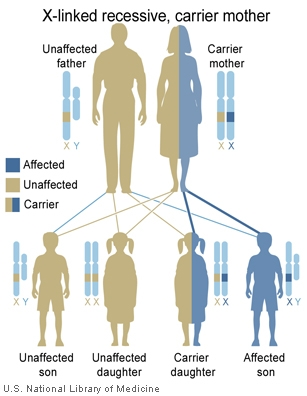
\includegraphics[width=0.5\textwidth]{figuraHerancaDaltonismo.jpg}
\caption{Herança de daltonismo. (retirado de \citeonline{ghrnlm2014}) \label{fig:figuraHerancaDaltonismo}}
\end{figure}

Os receptores responsáveis por identificar as cores são os cones e os bastonetes. Eles estão localizados na retina dos olhos. Os bastonetes funcionam como receptores acromáticos e os cones funcionam como receptores capazes de identificar cores. A Figura  \ref{fig:figuraOlhoHumano} ilustra onde a retina está localizada nos olhos e qual é a estrutura dos cones e bastonetes (em inglês, rods) na retina.

\begin{figure}[!htb]
\centering 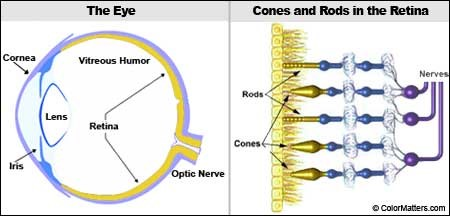
\includegraphics[width=0.5\textwidth]{figuraOlhoHumano.jpg}
\caption{O olho humano e os cones e bastonetes na retina do olho humano. (retirado de \citeonline{nigam2013}) \label{fig:figuraOlhoHumano}}
\end{figure}

Uma cor emite uma frequência de onda. O olho humano é capaz de identificar cores no intervalo de aproximadamente 400nm e 700nm. Abaixo dessa frequência estão os raios UV e acima dessa frequência estão os infra vermelhos. Essas e outras características podem ser visualizadas na Figura \ref{fig:figuraSpectro}.

\begin{figure}[!htb]
\centering
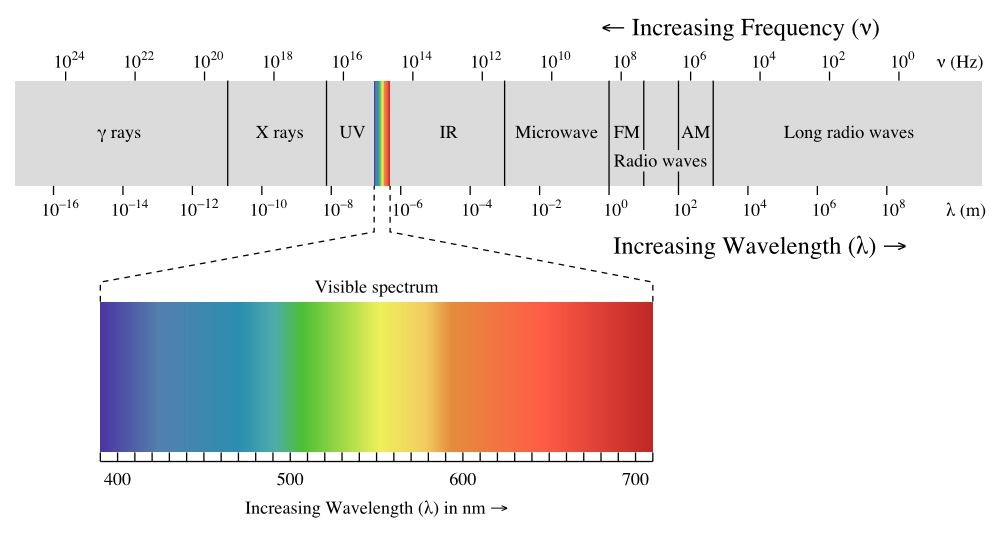
\includegraphics[width=0.9\textwidth]{figuraSpectro.jpg}
\caption{Espectro de frequência visível ao olho humano. (retirado de \citeonline{bolvan2014}) \label{fig:figuraSpectro}}
\end{figure}

Para identificar as cores, existem três tipos de sensores:

\begin{itemize}
\item Os cones do tipo L, que são os responsáveis em capturar ondas longas, cerca de 560 nanômetros, e identificam a cor vermelha;
\item Os cones do tipo M, que são os responsáveis em capturar ondas médias, cerca de 530 nanômetros, e identificam a cor verde;
\item Os cones do tipo S, que são os responsáveis em capturar ondas curtas, cerca de 420 nanômetros, e identificam a cor azul.
\end{itemize}

A Figura \ref{fig:figuraSensibilidadeCones} ilustra a provável porcentagem de absorção de cada tipo de cone na frequência visível aos seres humanos, onde a linha tracejada representa a frequência a qual os bastonetes são sensíveis e sua porcentagem de absorção e as linhas azul, verde e vermelha representam a frequência a qual os cones de tipo S, M e L são sensíveis e suas porcentagens de absorção, respectivamente. Essa representação é provável porque varia de pessoa para pessoa e a frequência visível por cada tipo de cone de um ser humano não pode ser calculada precisamente.

\begin{figure}[!htb]
\centering 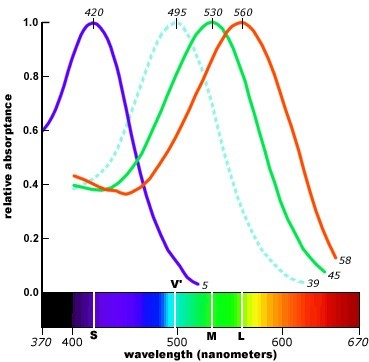
\includegraphics[width=0.5\textwidth]{figuraSensibilidadeCones.jpg}
\caption{Sensibilidade dos cones do olho humano. (retirado de \citeonline{bolvan2014}) \label{fig:figuraSensibilidadeCones}}
\end{figure}

\section{Tipos de daltonismo}
\label{sec:tiposDaltonismo}
Pessoas daltônicas possuem alguma deficiência nos cones. É possível classificá-los em três tipos: Os monocromatas, os dicromatas e os portadores de daltonismo do tipo tricomacia anômala. A Tabela \ref{tab:probabilidadeDaltonismo} apresenta o percentual aproximado de mulheres e homens daltônicos para cada um dos subtipos existentes e a seguir serão apresentados detalhes de cada um dos tipos e subtipos de daltonismo.


\begin{table}[h]
\centering
\begin{tabular}{|L{10em} |C{6em} |C{6em}|}
\hline      

\textbf{Tipo de daltonismo} & \textbf{Homens (\%)}  & \textbf{Mulheres (\%)}      \\ \hline
Protanopia                  & 1            & 0,02               \\ \hline
Protanomalia                & 1,5          & 0,03               \\ \hline
Deuteranopia                & 1            & 0,01               \\ \hline
Deuteranomalia              & 5            & 0,40               \\ \hline
Tritanopia/tritanomalia     & Muito raras  & Muito raras        \\ \hline
\end{tabular}
\caption{Prevalência dos tipos de defeitos congênitos na população masculina e feminina (retirado de \citeonline{bruni2006})}
\label{tab:probabilidadeDaltonismo}
\end{table}


\subsection{Monocromata}

As retinas das pessoas que possuem esse tipo de daltonismo, não possui nenhum ou apenas um tipo de cone. Daltônicos monocromatas não conseguem visualizar nenhuma cor, enxergam apenas tons de cinzas (preto, cinza e branco).

\subsection{Dicromata}
Ocorre quando um indivíduo não possui um tipo de cone. Os subtipos desse tipo de daltonismo são:

\begin{itemize}
\item Protanopia: Se o indivíduo não possui cones do tipo L, ou seja, quando não se é capaz de interpretar as ondas longas com precisão, as ondas que capturam a cor vermelha;
\item Deuteranopia: Se o indivíduo não possui cones do tipo M, ou seja, quando não se é capaz de interpretar as ondas médias com precisão, as ondas que capturam a cor verde;
\item Tritanopia: Se o indivíduo não possui cones do tipo S, ou seja, quando não se é capaz de interpretar as ondas curtas com precisão, as ondas que capturam a cor azul.
\end{itemize}

\subsection{Tricomacia Anômala}

Os indivíduos com esse tipo de daltonismo possuem os três tipos de cones. Porém, um tipo tem leve alteração de alinhamento e isso faz com que o indivíduo não consiga identificar as cores corretamente. Os subtipos desse tipo de daltonismo são:

\begin{itemize}
\item Protanomalia: cones do tipo L são defeituosos.
\item Deuteranomalia: cones do tipo M são defeituosos.
\item Tritanomalia: cones do tipo S são defeituosos.
\end{itemize}

\subsection{Daltonismo vermelho-verde}
Esse tipo de daltonismo ocorre quando os cones do tipo vermelho e/ou verde não capturam as frequência de cores corretamente. Daltonismo vermelho-verde é um termo utilizado para as subclassificações Protanopia, Deuteranopia, Protanomalia e Deuteranomalia.

\subsection{Daltonismo azul-amarelo}
Esse tipo de daltonismo ocorre quando os cones que identificam azul não capturam as frequências de cores corretamente. Daltonismo azul-amarelo é um termo utilizado para as subclassificações Tritanopia e Tritanomalia.

\section{Testes de daltonismo}
Vários testes de daltonismo já foram desenvolvidos. No entanto, a maioria desses testes se limita a identificar se uma pessoa possui problemas para diferenciar cores, não definindo qual é o subtipo exato de um daltônico.

\subsection{Ishahara}
\label{subsection:Ishihara}
 O teste de \citeonline{ishihara1917} é utilizado para identificar se pessoas possuem uma deficiência do tipo vermelho-verde. Criado por Dr. Shinobu Ishihara em 1917 na Universidade de Tóquio, esse teste consiste em identificar um número, ou quantidade de linhas em pranchas que são compostas por vários círculos coloridos.
Existem quatro tipos de pranchas:
\begin{itemize}
\item \textbf{Fuga}: apenas pessoas com visões normais conseguem visualizar o número ou uma quantidade de linhas e pessoas com daltonismo vermelho-verde não conseguem visualizar nada. Considerando o exemplo da Figura  \ref{fig:figuraIshiharaFuga}, pessoas com visão normal visualizam o número 45, enquanto pessoas com daltonismo vermelho-verde não veem nada.

\begin{figure}[!htb]
\centering 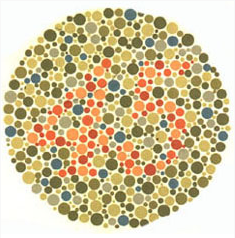
\includegraphics[width=0.5\textwidth]{figuraIshiharaFuga.png}
\caption{Teste de Ishihara, exemplo do tipo fuga. (retirado de \citeonline{colorblindnesssite}) \label{fig:figuraIshiharaFuga}}
\end{figure}
 
\item \textbf{Transformação}: pessoas com daltonismo vermelho-verde visualizam um número ou uma quantidade de linhas diferente da que é vista por pessoas com visão normal. A Figura \ref{fig:figuraIshiharaTransformacao} mostra um exemplo onde pessoas com visão normal visualizam o número 8 e pessoas com daltonismo vermelho-verde visualizam o número 3.
 
\begin{figure}[!htb]
\centering 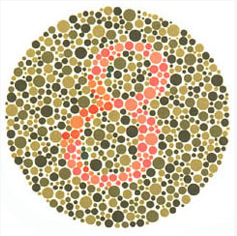
\includegraphics[width=0.5\textwidth]{figuraIshiharaTransformacao.png}
\caption{Teste de Ishihara, exemplo do tipo transformação. (retirado de \citeonline{colorblindnesssite}) \label{fig:figuraIshiharaTransformacao}}
\end{figure}

\item \textbf{Dígito escondido}: apenas daltônicos conseguem visualizar o número ou linha contida na prancha. Pessoas com visão normal não conseguem visualizar nada. Considerando o exemplo da Figura \ref{fig:figuraIshiharaEscondido}, pessoas com daltonismo vermelho-verde visualizam o número 5 e pessoas com visão normal não visualizam nada.

\begin{figure}[!htb]
\centering 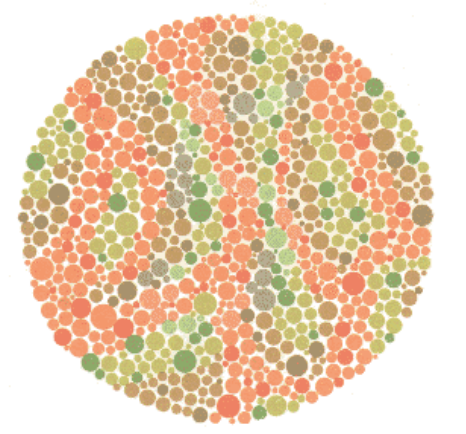
\includegraphics[width=0.5\textwidth]{figuraIshiharaEscondido.png}
\caption{Teste de Ishihara, exemplo do tipo dígito escondido. (retirado de \citeonline{colorblindnesssite}) \label{fig:figuraIshiharaEscondido}}
\end{figure}
 
\item \textbf{Classificação}: utilizado para identificar se o daltônico possui deficiência nos cones do tipo vermelho ou nos cones do tipo verde. Conforme o exemplo da Figura \ref{fig:figuraIshiharaClassificacao}, daltônicos do tipo Protanopia ou Protanomalia visualizam o número 2 perfeitamente, mas veem o número 4 de forma embaçada. Daltônicos do tipo Deuteranopia ou Deuteranomalia visualizam o número 4 perfeitamente, entretanto veem o número 2 embaçado.
 
\begin{figure}[!htb]
\centering 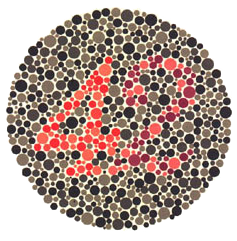
\includegraphics[width=0.5\textwidth]{figuraIshiharaClassificacao.png}
\caption{Teste de Ishihara, exemplo do tipo classificação. (retirado de \citeonline{colorblindnesssite}) \label{fig:figuraIshiharaClassificacao}}
\end{figure}

\end{itemize}

Outros exemplos de pranchas do teste de Ishihara podem ser visualizados no Apêndice \ref{ap:ishihara}.

\subsection{Teste de ordenação de cores}

Para executar esse teste, uma pessoa deve ordenar cores com base em uma cor inicial. O objetivo é realizar a ordenação de forma que a diferença entre as cores vizinhas seja a menor possível.

Existem diversas versões desse tipo de teste. A mais conhecida é a \textbf{Farnsworth D-15 arragement test}, onde a pessoa que está realizando o teste deve ordenar 15 cores seguindo a lógica de que as cores vizinhas devem ter a menor diferença possível. A Figura \ref{fig:figuraTesteOrdenacao} exibe um exemplo desse teste.

\begin{figure}[!htb]
\centering 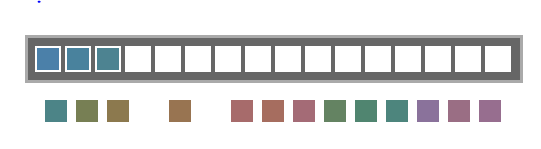
\includegraphics[width=0.8\textwidth]{figuraTesteOrdenacao.png}
\caption{Teste de ordenação de cores. (retirado de \citeonline{colorblindnesssite}) \label{fig:figuraTesteOrdenacao}}
\end{figure}

A seguir será apresentado a definição do que é uma imagem digital. Definição essencial para o processamento de imagens que será realizado para conseguir obter o objetivo deste trabalho.

\section{O que é uma imagem digital?}

Uma imagem digital em tons de cinza pode ser representada por uma matriz de inteiros onde a quantidade de brilho em cada pixel da imagem é armazenada em cada uma das posições da matriz. Nesse caso, quanto maior o número de linhas e colunas da matriz, maior a resolução da imagem. Além disso, quanto maior a quantidade de valores possíveis que um pixel pode assumir, maior a quantidade de níveis de cinza. Estas quantidades determinam a qualidade da imagem.

Para representar uma imagem colorida digitalmente, normalmente se utiliza mais de uma matriz. No caso do sistema de cores RGB (vermelho, verde e azul, do inglês red, green and blue), utiliza-se três matrizes com a mesma quantidade de linhas e colunas. Com isso, é possível armazenar a quantidade de vermelho, verde e azul em cada pixel da imagem. Na próxima seção serão apresentados mais detalhes a respeito de alguns sistemas de cores.

\section{Sistemas de cores}

O objetivo de um sistema de cores é definir um padrão para representação das cores. Trata-se de uma abstração da realidade. Em geral, os sistemas de cores são representados por sistemas tridimensionais onde cada coordenada representa uma cor.

O sistema de cores mais utilizado atualmente em monitores e câmeras digitais é o RGB. Esse sistema utiliza as cores primárias vermelho, verde e azul como base. Por outro lado, o sistema CMY (ciano, magenta e amarelo, do inglês cyan, magenta and yellow), que utiliza as cores secundárias ciano, magenta e amarelo, é mais utilizado em impressoras. 

Os sistema de cores HSI (matiz\footnote{Matiz: Conjunto de cores diversas bem combinadas; cada uma das gradações de uma cor; variedade de colorido. \cite{aurelioonline}}, saturação e intensidade, do inglês hue, saturation and intensity) e HSV (matiz, saturação e valor, do inglês hue, saturation and value) são mais próximos ao sistema visual humano do que os sistemas de cores RGB e CMY, porque a identificação de uma cor no sistema visual humano não é realizada apenas através da composição de três cores básicas. Uma cor é definida pela composição de matiz, saturação e brilho. A seguir são apresentados mais detalhes dos sistemas de cores RGB, CMY, HSI e HSV.

\subsection{RGB}

O sistema de cores RGB pode ser visualizado na Figura \ref{fig:figuraRGB}. Esse sistema consiste em um sistema cartesiano de três dimensões onde as dimensões são formadas pelas cores vermelha, verde e azul. Cada coordenada $(x_1, x_2, x_3)$ desse sistema representa uma cor, sendo $x_1$ a quantidade de vermelho presente na cor, $x_2$ a quantidade de verde e $x_3$ a quantidade de azul.

\begin{figure}[!htb]
\centering 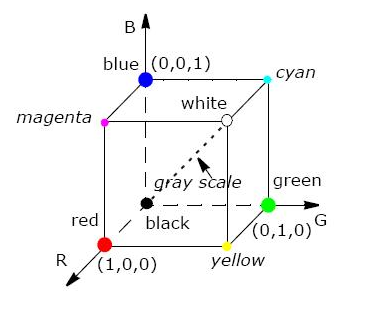
\includegraphics[width=0.7\textwidth]{figuraRGB.png}
\caption{O sistema de cores RGB. (retirado de \citeonline{cyberscience2014}) \label{fig:figuraRGB}}
\end{figure}

Conforme ilustrado na Figura \ref{fig:figuraFormacaoImagemRGB}, uma imagem no sistema RGB pode ser separada em três imagens em tons de cinza. Cada uma dessas três imagens representa a quantidade de vermelho, verde e azul que a imagem composta por essas três camadas possui.

\begin{figure}[!htb]
\centering 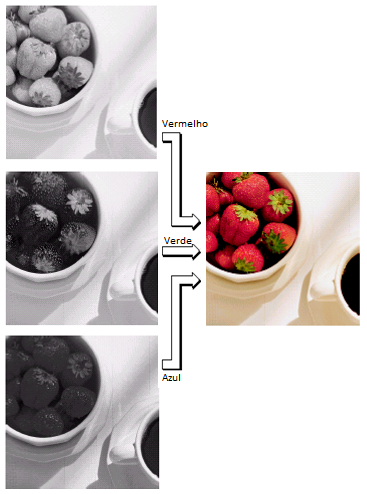
\includegraphics[width=0.7\textwidth]{figuraFormacaoImagemRGB.png}
\caption{Formação de uma imagem RGB. (adaptado de \citeonline{gonzalez2008}) \label{fig:figuraFormacaoImagemRGB}}
\end{figure}

\subsection{CMY}
O sistema de cores CMY é muito utilizado por impressoras. As dimensões desse sistema de cores são definidas pelas cores ciano, magenta e amarela. Na Figura \ref{fig:figuraCMY} é possível visualizar esse sistema de cores. 

\begin{figure}[!htb]
\centering 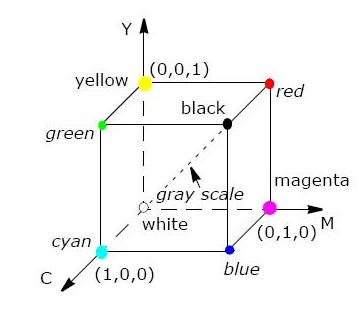
\includegraphics[width=0.5\textwidth]{figuraCMY.png}
\caption{O sistema de cores CMY. (retirado de \citeonline{cyberscience2014}) \label{fig:figuraCMY}}
\end{figure}

A conversão do sistema de cores RGB para o CMY é definida pela equação:

\begin{equation}
\left(\begin{array}{r}
C\\M\\Y
\end{array}\right)
=
\left(\begin{array}{r}
1\\1\\1
\end{array}\right)
-
\left(\begin{array}{r}
R\\G\\B
\end{array}\right)
\label{eq:CMY}
\end{equation}

Analogamente, a conversão do sistema de cores CMY para o sistema de cores RGB é realizada através da equação:

\begin{equation}
\left(\begin{array}{r}
R\\G\\B
\end{array}\right)
=
\left(\begin{array}{r}
1\\1\\1
\end{array}\right)
-
\left(\begin{array}{r}
C\\M\\Y
\end{array}\right)
\end{equation}

\subsection{HSI}

A Figura \ref{fig:figuraHSI} apresenta uma possível representação gráfica do sistema de cores HSI.

\begin{figure}[!htb]
\centering 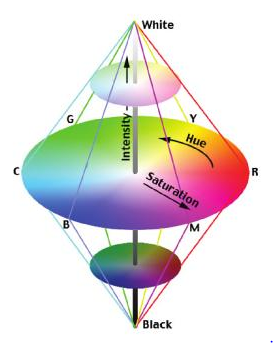
\includegraphics[width=0.5\textwidth]{figuraHSI.png}
\caption{O sistema de cores HSI. (retirado de \citeonline{russ2011}) \label{fig:figuraHSI}}
\end{figure}

É possível converter uma coordenada que está no sistema RGB para o sistema HSI. A matiz caracteriza a quantidade de cor contida em uma coordenada e pode ser obtido por:

\begin{equation}
H=\left\{\begin{array}{rc}
\delta,&\mbox{se}\quad B\leq G,\\
360 - \delta, &\mbox{se}\quad B>G.
\end{array}\right.
\end{equation}

sendo,
\begin{equation}
\delta = arccos \left( \frac{(R - G) + (R - B)}{2  \times  \sqrt{(R-G)^2 + (R-B)(G-B)} } \right)
\end{equation}
 
A saturação representa a quantidade de cor pura na coordenada e pode ser obtida por: 

\begin{equation}
S = 1 -  \frac{3 \times min(R, G, B)}{(R+G+B)} 
\end{equation}

A intensidade corresponde a quantidade de brilho relativo na coordenada e pode ser obtida por:

\begin{equation}
I = \frac{R+G+B}{3}
\end{equation}

É possível também converter cores que estão no sistema de cores HSI para o sistema de cores RGB. No entanto esse processo é mais complicado do que a conversão de RGB para HSI. De acordo com as equações para conversão de RGB para HSI, a matiz $H$ assume valores entre $0^o$ e $360^o$. A conversão de HSI para RGB é calculada de três formas diferentes, dependendo do valor de $H$. 

Se $0^o \leq H < 120^o$, então

\begin{equation}
B=I \times (1-S)
\end{equation}

\begin{equation}
R=I  \times \left( 1 +  \frac{S \times cosH}{cos (60^o - H)} \right)
\end{equation}

 e
\begin{equation}
G=3 \times I - (R+B).
\end{equation}

Se $120^o \leq H < 240^o$, devemos subtrair $120^o$ de H:

\begin{equation}
H=H-120^o
\end{equation}

e obter os componentes RGB através das equações

\begin{equation}
R=I \times (1-S)
\end{equation}

\begin{equation}
G=I  \times \left( 1 +  \frac{S \times cosH}{cos (60^o - H)} \right)
\end{equation}

e

\begin{equation}
B=3 \times I-(R+G).
\end{equation}

Por fim, se $240^0 \leq H \leq 360^o$, devemos subtrair $240^o$ de H:

\begin{equation}
H=H-240^o
\end{equation}

e obter os componentes RGB através das equações

\begin{equation}
G=I \times (1-S)
\end{equation}

\begin{equation}
B=I  \times \left( 1 +  \frac{S \times cosH}{cos (60^o - H)} ) \right)
\end{equation}

e

\begin{equation}
R=3 \times I-(G+B).
\end{equation}

As Figuras \ref{fig:figuraCuboRGB}, \ref{fig:figuraComponentesHSI} e \ref{fig:figuraComponentesHSI2} ilustram imagens no sistema RGB e no sistema HSI, para que seja possível compreender melhor o que cada um dos parâmetros do sistema HSI representa em uma imagem. Cada Figura é composta pela imagem no sistema RGB e as componentes matiz, saturação e intensidade da imagem.

\begin{figure}[!htb]
\centering 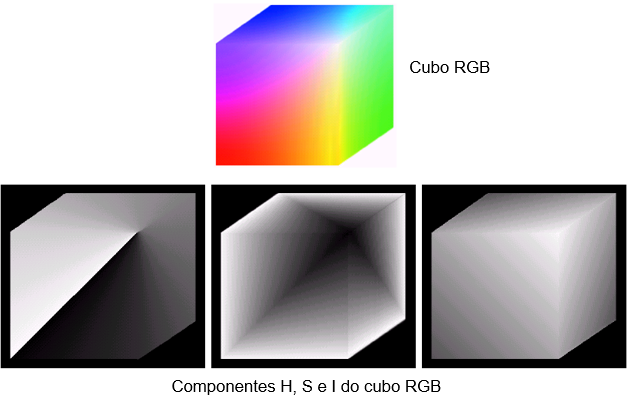
\includegraphics[width=0.5\textwidth]{figuraCuboRGB.png}
\caption{Componentes H, S e I do cubo RGB. (retirado de \citeonline{gonzalez2008}) \label{fig:figuraCuboRGB}}
\end{figure}

\begin{figure}[!htb]
\centering 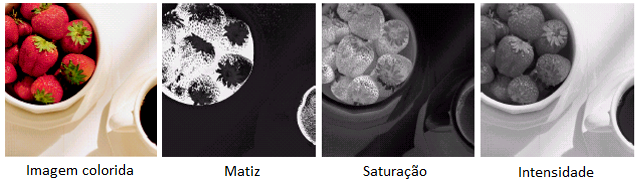
\includegraphics[width=\textwidth]{figuraComponentesHSI.png}
\caption{Componentes H, S e I de uma imagem RGB. (adaptado de \citeonline{gonzalez2008}) \label{fig:figuraComponentesHSI}}
\end{figure}

\begin{figure}[!htb]
\centering 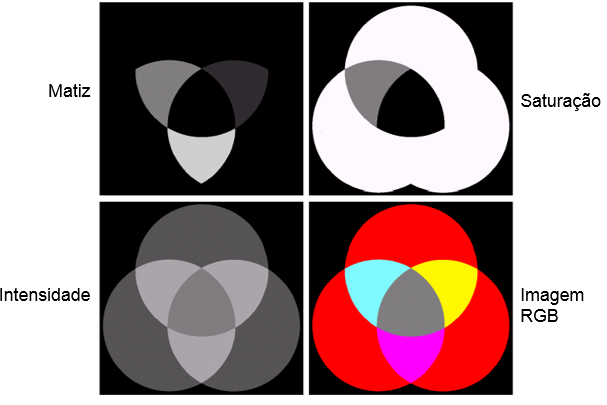
\includegraphics[width=0.5\textwidth]{figuraComponentesHSI2.png}
\caption{Imagem RGB das componentes H, S e I. (adaptado de \citeonline{gonzalez2008}) \label{fig:figuraComponentesHSI2}}
\end{figure}

\subsection{HSV}

O sistema de cores HSV também é denotado por HSB (matriz, saturação e brilho, do inglês hue, saturantion and brightness)\cite{burger2009digital}. A Figura \ref{fig:figuraHSV} apresenta uma possível representação gráfica do desse sistema de cores, a Figura \ref{fig:figuraHSV2} ilustra a posição de algumas cores dentro desse sistema e a Tabela \ref{tab:exemploHSV} lista os valores dos pontos que estão na Figura \ref{fig:figuraHSV2}.

\begin{figure}[!htb]
\centering 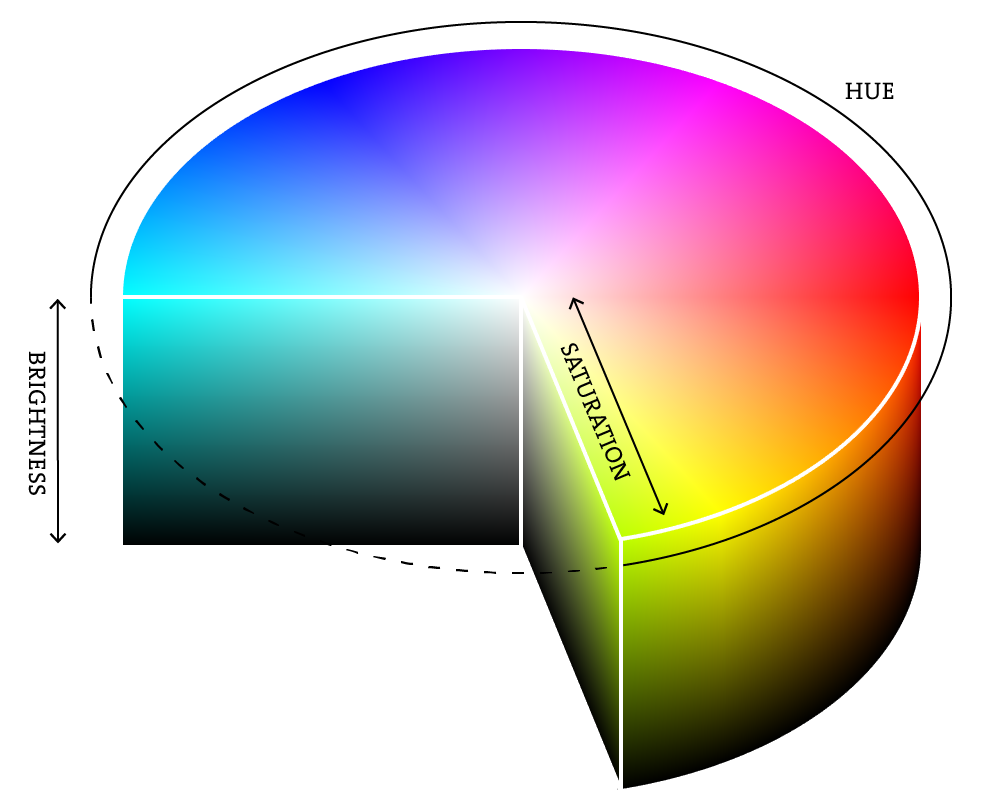
\includegraphics[width=0.5\textwidth]{figuraHSV.png}
\caption{O sistema de cores HSV, també conhecido como HSB. (retirado de \citeonline{processing}) \label{fig:figuraHSV}}
\end{figure}

\begin{figure}[!htb]
\centering 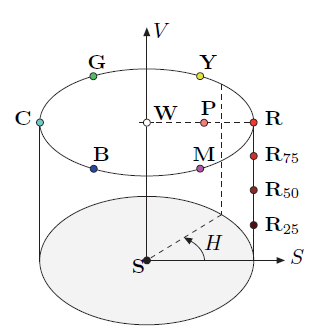
\includegraphics[width=0.5\textwidth]{figuraHSV2.png}
\caption{Posição de cores dentro do sistema de cores HSV. (retirado de \citeonline{burger2009digital}) \label{fig:figuraHSV2}}
\end{figure}

\begin{table}[h]
\centering
\begin{tabular}{clcccccc}
\hline      

\textbf{Ponto} & \textbf{Cor}              & \textbf{R} & \textbf{G} & \textbf{B} & \textbf{H} & \textbf{S} & \textbf{V}      \\ \hline
            S 	& Preto 		&0.00 	&0.00 	&0.00 	&— 	&0.00 	&0.00	\\ \hline
            R 	& Vermelho 		&1.00 	&0.00 	&0.00 	&0 	&1.00 	&1.00	\\ \hline
            Y 	&Amarelo 	&1.00 	&1.00 	&0.00 	&1/6 &1.00 	&1.00	\\ \hline
            G 	&Verde 		&0.00 	&1.00 	&0.00 	&2/6 &1.00 	&1.00	\\ \hline
            C 	&Ciano 		&0.00 	&1.00 	&1.00 	&3/6 &1.00 	&1.00	\\ \hline
            B 	&Azul 		&0.00 	&0.00 	&1.00 	&4/6 &1.00 	&1.00	\\ \hline
            M 	&Magenta 	&1.00 	&0.00 	&1.00 	&5/6 &1.00 	&1.00	\\ \hline
            W 	&Branco 		&1.00 	&1.00 	&1.00 	&— 	&0.00 	&1.00	\\ \hline
            $R_75$ &75\% Vermelho 	&0.75 	&0.00 	&0.00 	&0 	&1.00 	&0.75	\\ \hline
            $R_50$ &50\% Vermelho 	&0.50 	&0.00 	&0.00 	&0 	&1.00 	&0.50	\\ \hline
            $R_25$ &25\% Vermelho 	&0.25 	&0.00 	&0.00 	&0 	&1.00 	&0.25	\\ \hline
            P 	&Rosa 		&1.00 	&0.50 	&0.50 	&0 	&0.5 	&1.00	\\ \hline

\end{tabular}
\caption{Valores dos pontos ilustrados na Figura \ref{fig:figuraHSV2} (adaptado de \citeonline{burger2009digital})}
\label{tab:exemploHSV}
\end{table}

Existem diferentes formas de converter uma imagem RGB para o sistema de cores HSV. A mais popular entre elas utiliza as Equações \ref{eq:rgb2hsvV}, \ref{eq:rgb2hsvS},  \ref{eq:rgb2hsvH} e \ref{eq:rgb2hsvHH}, onde $r$, $g$ e $b$ são definidos através das Equações \ref{eq:rgb2hsvrr}, \ref{eq:rgb2hsvgg} e \ref{eq:rgb2hsvbb}, respectivamente \cite{acharya2005image}.


\begin{equation}
\label{eq:rgb2hsvV}
V = max(r,g,b)
\end{equation}

\begin{equation}
\label{eq:rgb2hsvS}
S=\left\{
\begin{array}{rc}

    0,&\mbox{se}\quad V = 0 \\
    V - \frac{min(r,g,b)}{V},&\mbox{se}\quad V>0

\end{array}\right.
\end{equation}

\begin{equation}
\label{eq:rgb2hsvH}
H=\left\{
\begin{array}{rc}

    0^o,&\mbox{se}\quad S = 0 \\
    \frac{60^o \times (g-b)}{S \times V},&\mbox{se}\quad V=r \\
    60^o \times \left( 2 + \frac{(b-r)}{S \times V} \right),&\mbox{se}\quad V=g \\
    60^o \times \left( 4 + \frac{(r-g)}{S \times V} \right),&\mbox{se}\quad V=r

\end{array}\right.
\end{equation}

\begin{equation}
\label{eq:rgb2hsvHH}
    H=H+360^o, se \quad H < 0
\end{equation}

\begin{equation}
\label{eq:rgb2hsvrr}
    r = \frac{R}{R+G+B}
\end{equation}

\begin{equation}
\label{eq:rgb2hsvgg}
    g = \frac{G}{R+G+B}
\end{equation}

\begin{equation}
\label{eq:rgb2hsvbb}
    b = \frac{b}{R+G+B}
\end{equation}

A conversão do sistema HSV para o sistema RGB é realizada através das Equações \ref{eq:hsv2rgbK}, \ref{eq:hsv2rgbT}, \ref{eq:hsv2rgbX}, \ref{eq:hsv2rgbY}, \ref{eq:hsv2rgbZ} e \ref{eq:hsv2rgbRGB} \cite{moeslund2012introduction}.

\begin{equation}
\label{eq:hsv2rgbK}
    K = \left\lfloor \frac{H}{60^o} \right\rfloor\footnote{$\lfloor x \rfloor$ significa o piso de x, ou seja, o maior valor inteiro menor ou igual a x.}
\end{equation}

\begin{equation}
\label{eq:hsv2rgbT}
    T = \frac{H}{60^o} - K;
\end{equation}

\begin{equation}
\label{eq:hsv2rgbX}
    X = V \times (1 - S)
\end{equation}

\begin{equation}
\label{eq:hsv2rgbY}
    Y = V \times (1 - S \times T)
\end{equation}

\begin{equation}
\label{eq:hsv2rgbZ}
    Z = V \times (1 - S \times (1 - T))
\end{equation}

\begin{equation}
\label{eq:hsv2rgbRGB}
(R,G,B)=\left\{
\begin{array}{rc}

    (V,Z,X),&\mbox{se}\quad K = 0 \\
    (Y,V,X),&\mbox{se}\quad K = 1 \\
    (X,V,Z),&\mbox{se}\quad K = 2 \\
    (X,Y,V),&\mbox{se}\quad K = 3 \\
    (Z,X,V),&\mbox{se}\quad K = 4 \\
    (V,X,Y),&\mbox{se}\quad K = 5
    

\end{array}\right.
\end{equation}











\section{Processamento de imagens}

O processamento de imagens é realizado com diversas finalidades. Por exemplo, a compressão de imagens e a restauração de imagens. A compressão busca diminuir a quantidade de bits necessários para representar uma imagem, perdendo o mínimo de detalhes possível e a restauração busca eliminar imperfeições em uma imagem. 

As aplicações de processamento de imagens podem ser dividias em três níveis. O primeiro possui imagens como atributos de entrada e saída. Por exemplo, aumentar o brilho de uma imagem, alterar a resolução, aumentar o contraste e etc. O segundo nível, possui como entrada uma imagem e como saída dados relacionados a esta imagem. Alguns exemplos seriam a identificação de bordas, contornos e etc. O terceiro e mais avançado nível de processamento de imagens requer uma análise mais avançada da imagem e tem como objetivo buscar o sentido do conteúdo da imagem. A identificação de um texto que está dentro de uma imagem seria um exemplo desse nível de processamento. Fotografia, impressão, imagens de satélite, processamento de imagens biomédicas, detecção de faces ou objetos, biometria, são alguns exemplos de aplicações de processamento de imagens.

Motivado pelo fato de que os seres humanos identificam milhares de cores em seu sistema visual, existem dois tipos de processamentos de imagens relacionados com cores, o processamento de imagens em pseudocores e processamento de imagens coloridas.

\subsection{Processamento de imagens em pseudocores}
Este tipo de processamento consiste em atribuir cores a uma imagem monocromática com base em um determinado critério. Ou seja, dada uma imagem que possui apenas tons de cinza como entrada, a saída será uma imagem colorida.

\subsection{Processamento de imagens coloridas}

O processamento de imagens coloridas pode ser dividido em duas categorias. Em uma primeira categoria estão os métodos que processam cada componente de cor (e.g. os componentes vermelho, verde e azul) de uma imagem separadamente e depois de realizar o processamento combina esses componentes para formar a imagem colorida novamente. A outra categoria realiza o processamento da imagem diretamente na imagem colorida, sem separar os seus componentes.

\section{Simuladores de daltonismo}

Existe um algoritmo para simulação de daltonismo apresentado por \citeonline{Vienot1999}. Esse algoritmo utiliza o sistema de cores LMS (ondas longas, ondas médias e ondas pequenas, do inglês Longwave, Middlewave and Shortwave). A Figura \ref{fig:figuraSimulador} exibe imagens onde foram aplicados os filtros para daltônicos do tipo Protanopia e Deuteranopia. O primeiro passo desse algoritmo consiste em converter a imagem do sistema de cores RGB para o sistema LMS utilizando a multiplicação de matrizes \ref{eq:simulador1}.

\begin{equation}
\left(\begin{array}{ccc}
L\\M\\S
\end{array}\right)
=
\left(\begin{array}{ccc}
17,8824 & 43,5161 & 4,11935 \\
3,45565 & 27,1554 & 3,86714 \\
0,0299566 & 0,184309 & 1,46709
\end{array}\right)
\left(\begin{array}{ccc}
R\\G\\B
\end{array}\right)
\label{eq:simulador1}
\end{equation}

Após essa conversão, é necessário reduzir o domínio de cores. Para simular o daltonismo do tipo Protanopia, a redução é feita utilizando a multiplicação de matrizes \ref{eq:simulaProt}.

\begin{equation}
\left(\begin{array}{ccc}
L_1\\M_1\\S_1
\end{array}\right)
=
\left(\begin{array}{ccc}
0 & 2,23344 & -2,52581 \\
0 & 1 & 0 \\
0 & 0 & 1
\end{array}\right)
\left(\begin{array}{ccc}
L\\M\\S
\end{array}\right)
\label{eq:simulaProt}
\end{equation}

Para simular o daltonismo do tipo Deuteranopia, a redução é feita utilizando a multiplicação de matriz \ref{eq:simulaDeut}.

\begin{equation}
\left(\begin{array}{ccc}
L_1\\M_1\\S_1
\end{array}\right)
=
\left(\begin{array}{ccc}
1 & 0 & 0 \\
0,494207 & 0 & 1,24827 \\
0 & 0 & 1
\end{array}\right)
\left(\begin{array}{ccc}
L\\M\\S
\end{array}\right)
\label{eq:simulaDeut}
\end{equation}

\begin{figure}[!htb]
\minipage{0.32\textwidth}
\centering
{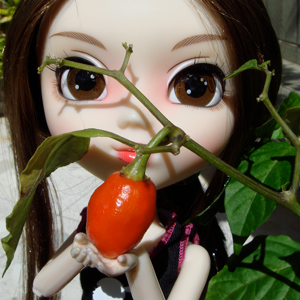
\includegraphics[width=\linewidth]{figuraSimuladorOriginal.png}}
(a)
\endminipage\hfill
\minipage{0.32\textwidth}
\centering
{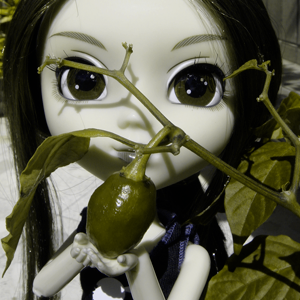
\includegraphics[width=\linewidth]{figuraSimuladorProtan.png}}
(b)
\endminipage\hfill
\minipage{0.32\textwidth}%
\centering
{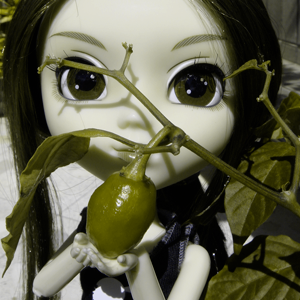
\includegraphics[width=\linewidth]{figuraSimuladorDeutan.png}}
(c)
\endminipage
\caption{Resultado de simulação. (a) Imagem original RGB, visão normal. (b) Imagem RGB simulando o daltonismo do tipo Protanopia. (c) Imagem RGB simulando o daltonismo do tipo Deuteranopia. (retirado de  \citeonline{jlee2008})}
\label{fig:figuraSimulador}
\end{figure}

Por fim, é necessário converter a imagem de volta para o sistema RGB. Para isso é necessário multiplicar a matriz resultante da multiplicação de matrizes realizada em \ref{eq:simulaDeut} ou \ref{eq:simulaProt} pela matriz inversa da que foi utilizada para converter a imagem do sistema RGB para o sistema LMS em \ref{eq:simulador1}.

\begin{equation}
\left(\begin{array}{ccc}
R_1\\G_1\\B_1
\end{array}\right)
=
\left(\begin{array}{ccc}
0,080944 & -0,130504 & 0,116721 \\
-0,0102485 & 0,0540194 & -0,113615 \\
-0,000365294 & -0,00412163 & 0,693513
\end{array}\right)
\left(\begin{array}{ccc}
L_1\\M_1\\S_1
\end{array}\right)
\label{eq:simulador2}
\end{equation}


\section{Ferramentas adaptativas para daltônicos}

O daltonismo é uma deficiência que até o momento não foi desenvolvida uma maneira para curá-la. No entanto, existem ferramentas de auxílio aos daltônicos que não possuem o objetivo de corrigir o daltonismo, possuem o objetivo de modificar ou filtrar as cores para que um daltônico consiga identificar as diferenças de cores com mais precisão. 
 
Foram encontrados alguns trabalhos com o objetivo de corrigir imagens para melhorar a identificação das cores por pessoas daltônicas. É possível classificar esses trabalhos em duas categorias: lentes para daltônicos e processamento de imagens. Detalhes de cada uma dessas categorias serão apresentadas a seguir.

\subsection{Lentes para daltônicos}

As lentes de contato para daltônicos possuem o objetivo de ajustar as cores para que seja possível identificar as diferenças de cores com mais precisão. Não há melhora para monocromatas que utilizam esse tipo de lente. Para daltônicos de outros tipos, melhoras consideráveis são apresentadas no teste de Ishihara e não há melhora no teste de ordenação de cores. 

Alguns fabricantes desse tipo de lente são \citeonline{colormax2012}, \citeonline{colorview2014} e \citeonline{chromagen2014}. Eles divulgam esse produto como a cura do daltonismo ou corretor de daltonismo, mas conforme citado anteriormente, isso não é possível. Não existem estudos que comprovem a eficiência desse produto no dia-a-dia de uma pessoa portadora de daltonismo.

\subsection{Processamento de imagens}

Como já foi apresentado anteriormente, uma imagem pode ser representada por $f(x,y)$ e o valor de $f(x,y)$ representa a cor contida na posição x e y da imagem. Pode-se alterar esse valor utilizando processamento de imagens e com o objetivo de realçar as diferenças entre as cores da imagem.

Utilizando as pranchas do teste de Ishihara, um modo extremo de realizar esse tipo de processamento é remover os componentes verde e azul da imagem e realçar o vermelho. Com esse processamento, os daltônicos conseguirão visualizar o que as pessoas com visão normal visualizam nas pranchas. No entanto, as pranchas resultantes são compostas apenas pela cor vermelha e diferem muito das cores inicias das pranchas, conforme é possível visualizar na Figura \ref{fig:figuraMatlab3} após a aplicação desse procedimento na Figura \ref{fig:figuraMatlab1}. 

Esse procedimento foi apresentado por \citeonline{kulshrestha} e pode ser facilmente executado no Matlab utilizando a função \ref{eq:imadjust}. Nesta função, a variável $R$ é a imagem resultante do procedimento e $E$ é a imagem de entrada.

\begin{equation}
R=imadjust (E,[0 \; 0 \; 0; 1 \; 1 \; 1],[1 \; 1 \; 1; 0 \; 0 \; 0],[2 \; 0 \; 0]) \label{eq:imadjust}
\end{equation}

\begin{figure}[!htb]
\centering 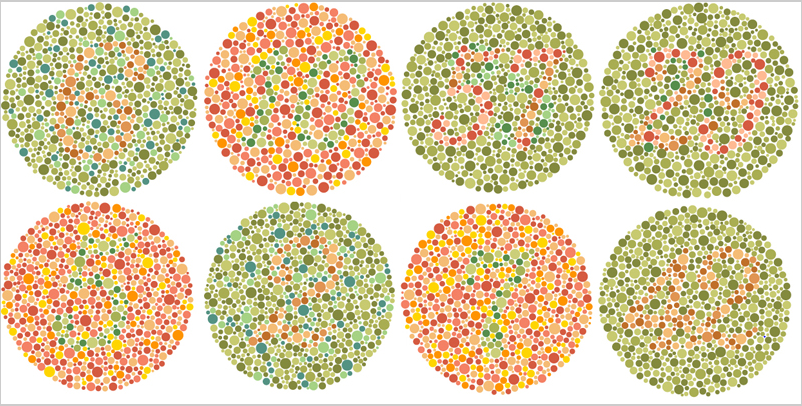
\includegraphics[width=0.7\textwidth]{figuraMatlab1.PNG}
\caption{Pranchas de Ishihara. \label{fig:figuraMatlab1}}
\end{figure}

\begin{figure}[!htb]
\centering 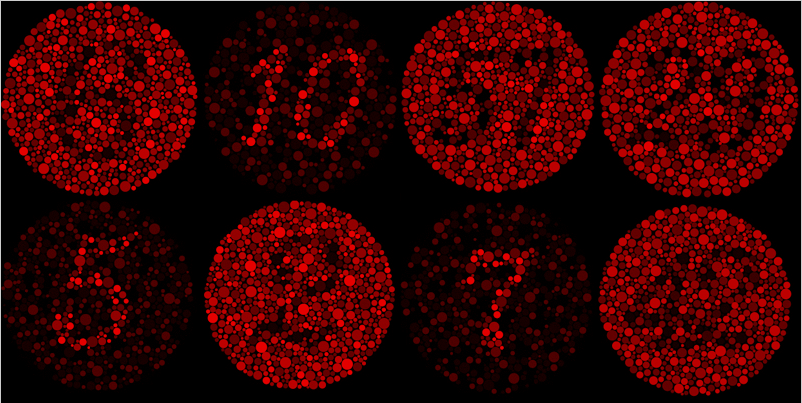
\includegraphics[width=0.7\textwidth]{figuraMatlab3.PNG}
\caption{Resultado do processamento \ref{eq:imadjust}. \label{fig:figuraMatlab3}}
\end{figure}


Outros trabalhos encontrados utilizam uma inteligência computacional maior para melhorar a visualização das imagens por daltônicos. \citeonline{jlee2008} apresentou no seu TCC uma sequência de processamentos de imagens para facilitar a visualização de imagens para pessoas portadoras de daltonismo. No processamento definido por ela, as componentes de cores recebem novos valores dependendo do tipo de daltonismo e utilizam como base as outras componentes de cores. Por exemplo, para os daltônicos do tipo Protanopia, os novos valores das componentes de cores verde e azul são definidos através da média entre os valores originais dessas componentes e os valores da componente vermelha, conforme a Equação \ref{eq:equacaojlee}. Também foi definido nesse trabalho uma maneira de equalizar as novas cores.

\begin{equation}
f^\prime =  (f_r, f_g^\prime, f_b^\prime), \left\{\begin{array}{rc}
f_g^\prime = \frac{f_r + f_g}{2}\\
f_b^\prime = \frac{f_r + f_b}{2}
\end{array}\right.
\label{eq:equacaojlee}
\end{equation}

No entanto, esse trabalho não apresentou bons resultados, conforme podemos visualizar na Figura \ref{fig:resultadosjlee}. Nessa figura, a imagem (a) é a imagem original, na imagem (b) é exibido o resultado com equalização e na imagem (c) o resultado sem equalização. A imagem não teve suas cores realçadas em nenhum dos dois resultados apresentados.

\begin{figure}[!htb]
\minipage{0.30\textwidth}
\centering
{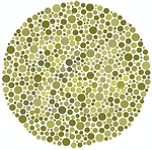
\includegraphics[width=\linewidth]{jleeoriginal.png}}
(a)
\endminipage\hfill
\minipage{0.30\textwidth}
\centering
{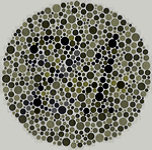
\includegraphics[width=\linewidth]{jleecomequalizacao.png}}
(b)
\endminipage\hfill
\minipage{0.30\textwidth}
\centering
{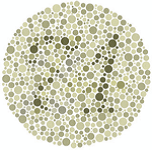
\includegraphics[width=\linewidth]{jleesemequalizacao.png}}
(c)
\endminipage\hfill
\caption{Resultado da correção da imagem (a) com equalização (b) e sem equalização (c). (retirado de \citeonline{jlee2008})}
\label{fig:resultadosjlee}
\end{figure}


A Figura \ref{fig:figuraChromophore} exibe a adaptação das imagens de Ishihara utilizando um aplicativo para Windows Phone 7 criado por \citeonline{chromophore2011}. Esse aplicativo e outros trabalhos semelhantes (\citeonline{wicaksana2011}, \citeonline{manaf2012}, \citeonline{ohkubo2008} e \citeonline{harwahyu2013}) apresentam melhores resultados e eles utilizam uma sequências de processamento semelhantes entre si para realçar as cores e facilitar a visualização de imagens por daltônicos. Esses trabalhos buscam melhorar a qualidade de imagens sem remover nenhuma componente de cor (vermelho, verde ou azul). Os processamentos de imagens feitos nesses trabalhos convertem as imagens para outros sistemas de cores, realizam procedimentos nesses outros sistemas e posteriormente convertem de volta para o sistema de cores original, conforme ilustrado no fluxograma da Figura \ref{fig:figFluxoCorrecao}.

Com a finalidade de facilitar a distinção de cores por daltônicos, \citeonline{chromophore2011} converteu a imagem para o sistema de cores HSI e alterou os valores da matiz e da intensidade nesse sistema. As alterações feitas na matiz a na intensidade não foram apresentadas no artigo, mas o resultados apresentados foram superiores aos que foram apresentados por \citeonline{jlee2008}.

\begin{figure}[!htb]
\centering 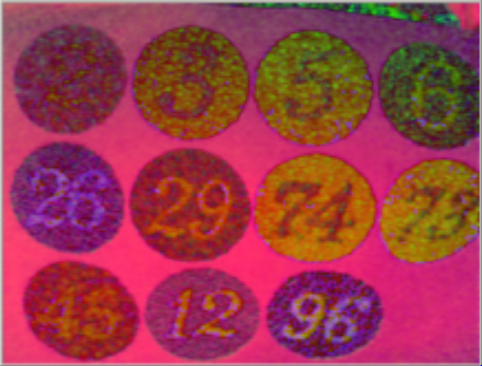
\includegraphics[width=0.6\textwidth]{figureChromophore.png}
\caption{Exibição do funcionamento do aplicativo. (adaptado de \citeonline{chromophore2011}) \label{fig:figuraChromophore}}
\end{figure}

\begin{figure}[!htb]
\centering 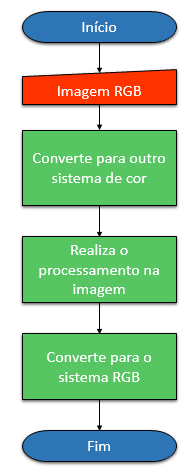
\includegraphics[width=0.30\textwidth]{figuraFluxoCorrecao.PNG}
\caption{Sequências de passos para realçar cores de uma imagem RGB. \label{fig:figFluxoCorrecao}}
\end{figure}

% ---
% Finaliza a parte no bookmark do PDF, para que se inicie o bookmark na raiz
% ---
\bookmarksetup{startatroot}% 
% ---

% ---
% Desenvolvimento
% ---
\chapter{Desenvolvimento}

\section{Escolha do sistema de cor}

A sequência descrita na Figura \ref{fig:figFluxoCorrecao} foi testada utilizando os sistemas de cores HSI e HSV. Foi escolhido processar as imagens nesses sistemas de cores porque eles se aproximam da maneira em que os seres humanos identificam as cores. 

Com isso, todas as tentativas de processamento para alcançar o objetivo deste trabalho se resumem em converter uma imagem RGB para o sistema de cores HSI ou HSV, realizar dado processamento e converter a imagem para de volta o sistema de cores RGB. Detalhes dos processamentos de imagens realizados nesses sistemas de cores serão apresentados na Seção \ref{sec:processamentoDasImagens}.

A ferramenta desenvolvida utiliza apenas um desses dois sistemas de cores. Inicialmente não era possível definir qual apresentaria resultado melhores, por isso foram realizados testes com ambos.


\section{Processamento das imagens}
\label{sec:processamentoDasImagens}

Afim de alcançar o objetivo desse trabalho, foram desenvolvidas duas abordagens diferentes. A primeira tem como principal objetivo \textbf{reduzir possíveis valores da matiz} e a segunda \textbf{elevar os valores da intensidade ou valor}, utilizando o sistema de cores HSI ou HSV. Essas abordagens serão descritas com detalhes nas Subseções \ref{subsec:deslocarH} e \ref{subsec:deslocarVouI}.

\subsection{Reduzir possíveis valores da matiz}
\label{subsec:deslocarH}

O componente H dos sistemas de cores HSI e HSV representa a matiz. A matiz é definida por um ângulo que está no intervalo $[0^o, 360^o]$. A Tabela \ref{tab:coresEmH} apresenta os ângulos de algumas cores nesse componente e a Figura \ref{fig:figuraColorsH} ilustra a posição dessas cores dentro de um círculo que representa os possíveis valores de H.


\begin{table}[h]
\centering
\begin{tabular}{clcccccc}
\hline      

\textbf{Ângulo}     & \textbf{Cor}  \\ \hline
$0^o$ / $360^o$     & Vermelho      \\ \hline
$30^o$              & Laranja       \\ \hline
$60^o$              & Amarelo       \\ \hline
$900^o$             & Oliva         \\ \hline
$120^o$             & Verde         \\ \hline
$150^o$             & Turquesa      \\ \hline
$180^o$             & Ciano         \\ \hline
$210^o$             & Celeste       \\ \hline
$240^o$             & Azul          \\ \hline
$270^o$             & Púrpura       \\ \hline
$300^o$             & Magenta       \\ \hline
$330^o$             & Rosa          \\ \hline

\end{tabular}
\caption{Ângulos de algumas cores no componente H dos sistemas de cores HSI e HSV.}
\label{tab:coresEmH}
\end{table}

\begin{figure}[!htb]
\centering 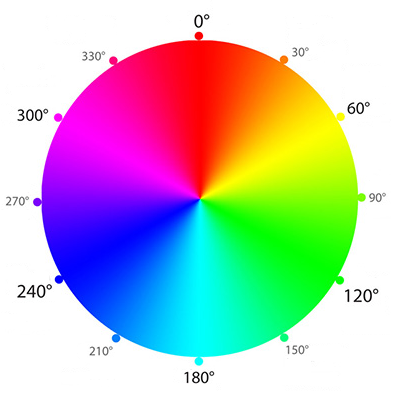
\includegraphics[width=0.60\textwidth]{figuraColorsH.PNG}
\caption{Matiz dos sistemas de cores HSI e HSV. (adaptado de \citeonline{onextrapixel}) \label{fig:figuraColorsH}}
\end{figure}

A maioria dos daltônicos visualizam as três cores primárias (vermelho, verde e azul) mas possuem deficiência em um tipo de cone, conforme foi apresentado no Seção \ref{sec:tiposDaltonismo}. 

Dado que os valores de H estão no intervalo $[0^o, 360^o]$ e que os ângulos pertencentes a H não necessitam ser inteiros, existem infinitos valores possíveis para H. Com o objetivo de facilitar a distinção de cores por daltônicos, o primeiro processamento de imagem executado neste trabalho reduz os possíveis valores de H para um conjunto finito de 3, 6 e 12 elementos.

A transformação de H para 3 elementos é realizada através da Equação \ref{eq:reduzirHpara3}, para 6 através da Equação \ref{eq:reduzirHpara6} e para 12 através da Equação \ref{eq:reduzirHpara12}. 

\begin{equation}
\label{eq:reduzirHpara3}
H'=\left\{
\begin{array}{rc}
    0^o,&\mbox{se}\quad H <60^o ou H \geq 300^o \\
    120^o,&\mbox{se}\quad H \geq 60^o e H < 180^o \\
    240^o,&\mbox{se}\quad H \geq 180^o e H < 300^o \\
\end{array}\right.
\end{equation}

\begin{equation}
\label{eq:reduzirHpara6}
H''=\left\{
\begin{array}{rc}
    0^o,&\mbox{se}\quad H <30^o ou H \geq 330^o \\
    60^o,&\mbox{se}\quad H \geq 30^o e H < 90^o \\
    120^o,&\mbox{se}\quad H \geq 90^o e H < 150^o \\
    180^o,&\mbox{se}\quad H \geq 150^o e H < 210^o \\
    240^o,&\mbox{se}\quad H \geq 210^o e H < 270^o \\
    300^o,&\mbox{se}\quad H \geq 270^o e H < 330^o \\
\end{array}\right.
\end{equation}

\begin{equation}
\label{eq:reduzirHpara12}
H'''=\left\{
\begin{array}{rc}
    0^o,&\mbox{se}\quad H <15^o ou H \geq 345^o \\
    30^o,&\mbox{se}\quad H \geq 15^o e H < 45^o \\
    60^o,&\mbox{se}\quad H \geq 45^o e H < 75^o \\
    90^o,&\mbox{se}\quad H \geq 75^o e H < 105^o \\
    120^o,&\mbox{se}\quad H \geq 105^o e H < 135^o \\
    150^o,&\mbox{se}\quad H \geq 135^o e H < 165^o \\
    180^o,&\mbox{se}\quad H \geq 165^o e H < 195^o \\
    210^o,&\mbox{se}\quad H \geq 195^o e H < 225^o \\
    240^o,&\mbox{se}\quad H \geq 225^o e H < 255^o \\
    270^o,&\mbox{se}\quad H \geq 255^o e H < 285^o \\
    300^o,&\mbox{se}\quad H \geq 285^o e H < 315^o \\
    330^o,&\mbox{se}\quad H \geq 315^o e H < 345^o \\
\end{array}\right.
\end{equation}

Aplicando a Equação \ref{eq:reduzirHpara3} nas imagens, elas serão transformadas em imagens em tons de vermelho, verde e azul. Aplicando a Equação \ref{eq:reduzirHpara6}, as imagens serão compostas por tons de vermelho, amarelo, verde, ciano, azul e magenta. Por fim, aplicando a Equação \ref{eq:reduzirHpara6}, as imagens serão compostas por tons de vermelho, laranja, amarelo, oliva, verde, turquesa, ciano, celeste, azul, púrpura, magenta e rosa.

A Figura \ref{fig:platesIshihara} foi processada utilizando as equações \ref{eq:reduzirHpara3}, \ref{eq:reduzirHpara6} e \ref{eq:reduzirHpara12}, separadamente. Os respectivos resultados são apresentados nas Figuras \ref{fig:reduzirHpara3}, \ref{fig:reduzirHpara6} e \ref{fig:reduzirHpara12}.

\begin{figure}[!htb]
\centering 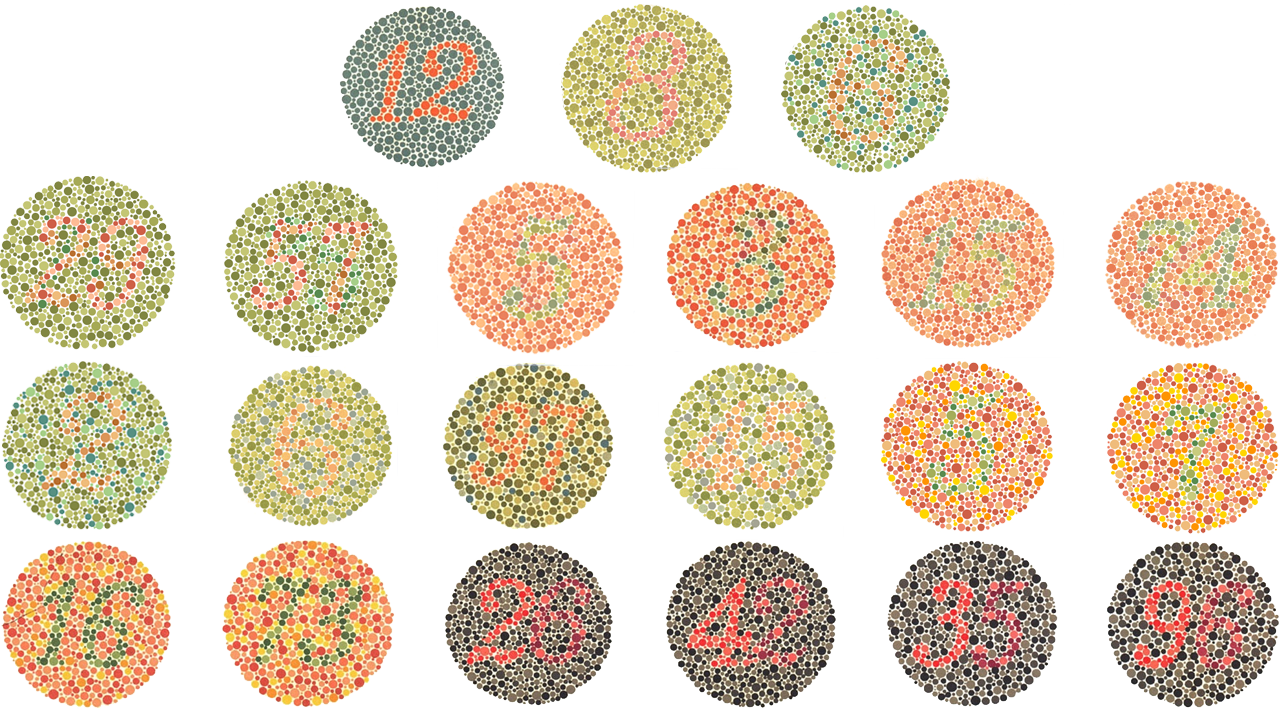
\includegraphics[width=0.90\textwidth]{platesIshihara.png}
\caption{Pranchas de Ishihara) \label{fig:platesIshihara}}
\end{figure}

\begin{figure}[!htb]
\centering 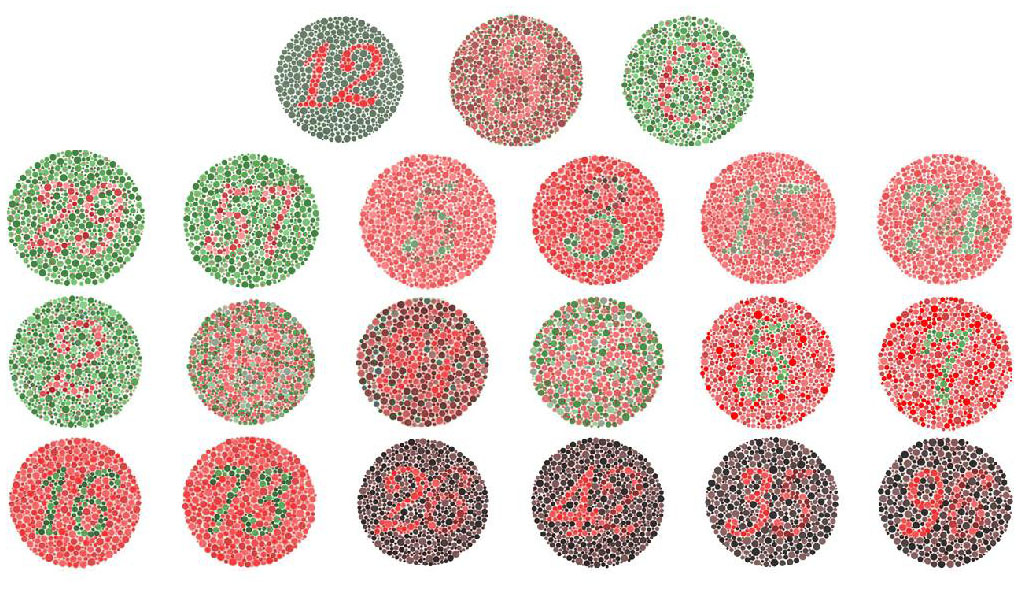
\includegraphics[width=0.90\textwidth]{figuraDeslocarH3.jpg}
\caption{Resultado da Equação \ref{eq:reduzirHpara3} sobre a Figura \ref{fig:platesIshihara}. \label{fig:reduzirHpara3}}
\end{figure}

\begin{figure}[!htb]
\centering 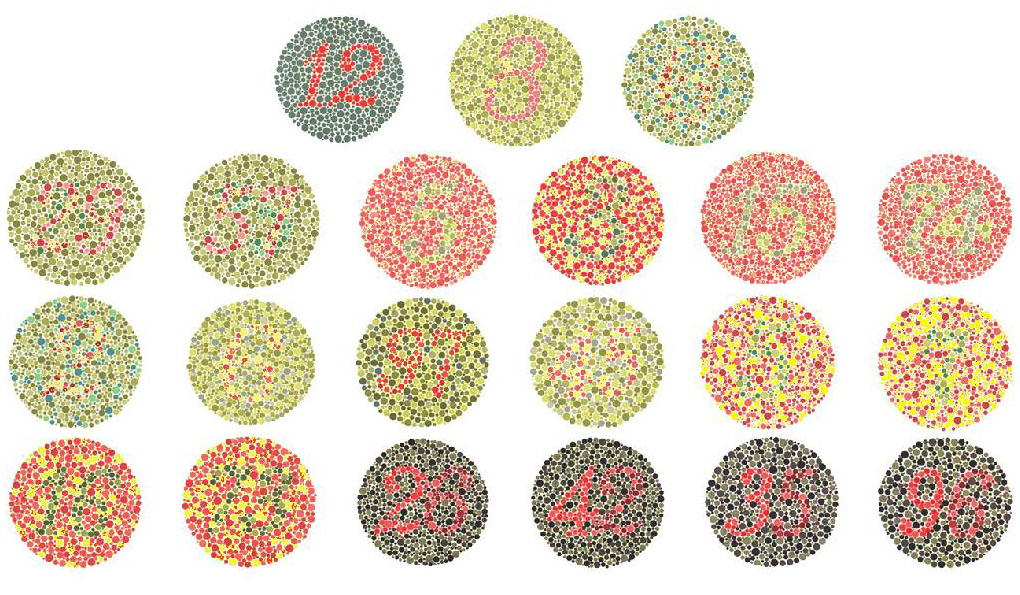
\includegraphics[width=0.90\textwidth]{figuraDeslocarH6.jpg}
\caption{Resultado da Equação \ref{eq:reduzirHpara6} sobre a Figura \ref{fig:platesIshihara}. \label{fig:reduzirHpara6}}
\end{figure}

\begin{figure}[!htb]
\centering 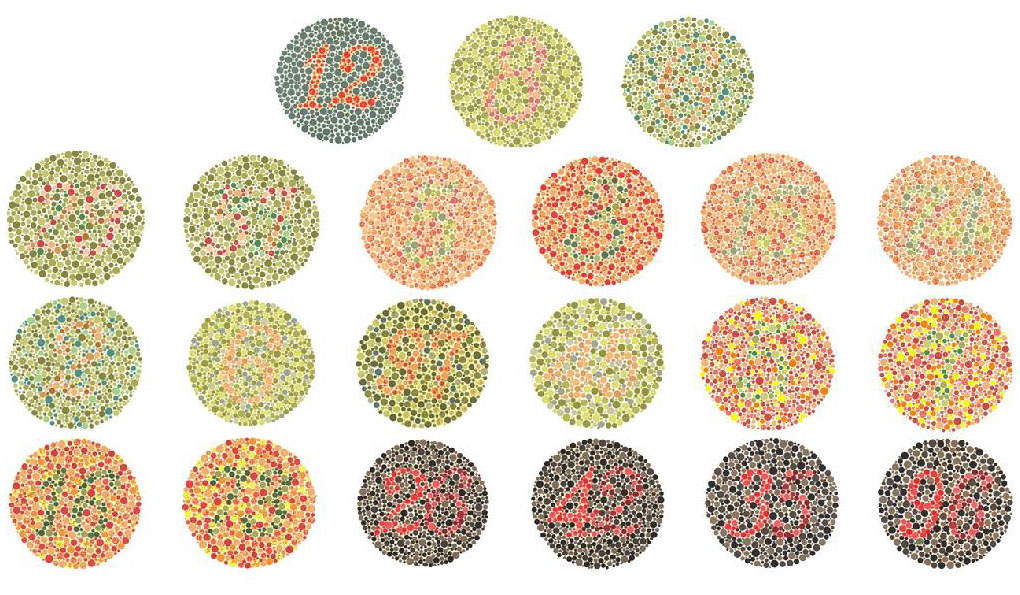
\includegraphics[width=0.90\textwidth]{figuraDeslocarH12.jpg}
\caption{Resultado da Equação \ref{eq:reduzirHpara12} sobre a Figura \ref{fig:platesIshihara}. \label{fig:reduzirHpara12}}
\end{figure}

Adicionalmente a redução de elementos do conjunto o qual H pertence, também foi implementado métodos de limitar os valores da saturação e do valor ou intensidade das imagens, conforme as equações \ref{eq:reduzirS}, \ref{eq:reduzirI} e \ref{eq:reduzirV}.

\begin{equation}
\label{eq:reduzirS}
S'=\left\{
\begin{array}{rc}
       0,&\mbox{se}\quad S <    \frac{1}{6}                               \\
    0.33,&\mbox{se}\quad S \geq \frac{1}{6} e S < \frac{3}{6}      \\
    0.66,&\mbox{se}\quad S \geq \frac{3}{6} e S < \frac{5}{6}      \\
       1,&\mbox{se}\quad S \geq \frac{5}{6}
\end{array}\right.
\end{equation}

\begin{equation}
\label{eq:reduzirI}
I'=\left\{
\begin{array}{rc}
       0,&\mbox{se}\quad I <    \frac{1}{6}                               \\
    0.33,&\mbox{se}\quad I \geq \frac{1}{6} e I < \frac{3}{6}      \\
    0.66,&\mbox{se}\quad I \geq \frac{3}{6} e I < \frac{5}{6}      \\
       1,&\mbox{se}\quad I \geq \frac{5}{6}
\end{array}\right.
\end{equation}

\begin{equation}
\label{eq:reduzirV}
V'=\left\{
\begin{array}{rc}
       0,&\mbox{se}\quad V <    \frac{1}{6}                               \\
    0.33,&\mbox{se}\quad V \geq \frac{1}{6} e V < \frac{3}{6}      \\
    0.66,&\mbox{se}\quad V \geq \frac{3}{6} e V < \frac{5}{6}      \\
       1,&\mbox{se}\quad V \geq \frac{5}{6}
\end{array}\right.
\end{equation}

A Figura \ref{fig:reduzirHSeV} ilustra a aplicação das equações \ref{eq:reduzirHpara3}, \ref{eq:reduzirS} e \ref{eq:reduzirV} sobre a Figura \ref{fig:platesIshihara} e a A Figura \ref{fig:reduzirHSeI} ilustra a aplicação das equações \ref{eq:reduzirHpara3}, \ref{eq:reduzirS} e \ref{eq:reduzirI} sobre a Figura \ref{fig:platesIshihara}.

\begin{figure}[!htb]
\centering 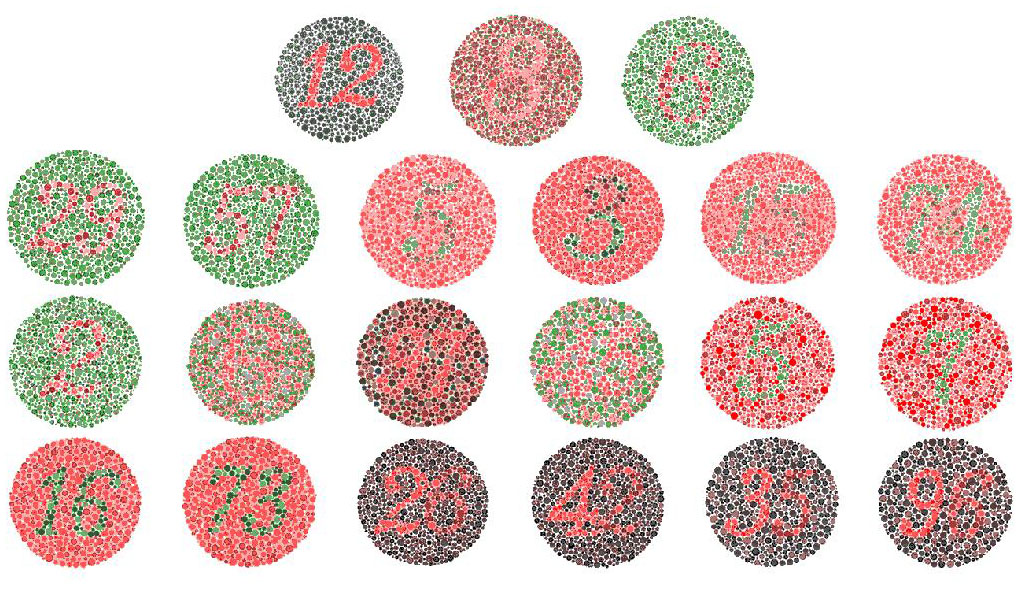
\includegraphics[width=0.90\textwidth]{figuraDeslocarHSeV.jpg}
\caption{Resultado da aplicação das Equações \ref{eq:reduzirHpara3}, \ref{eq:reduzirS} e \ref{eq:reduzirV} sobre a Figura \ref{fig:platesIshihara}. \label{fig:reduzirHSeV}}
\end{figure}

\begin{figure}[!htb]
\centering 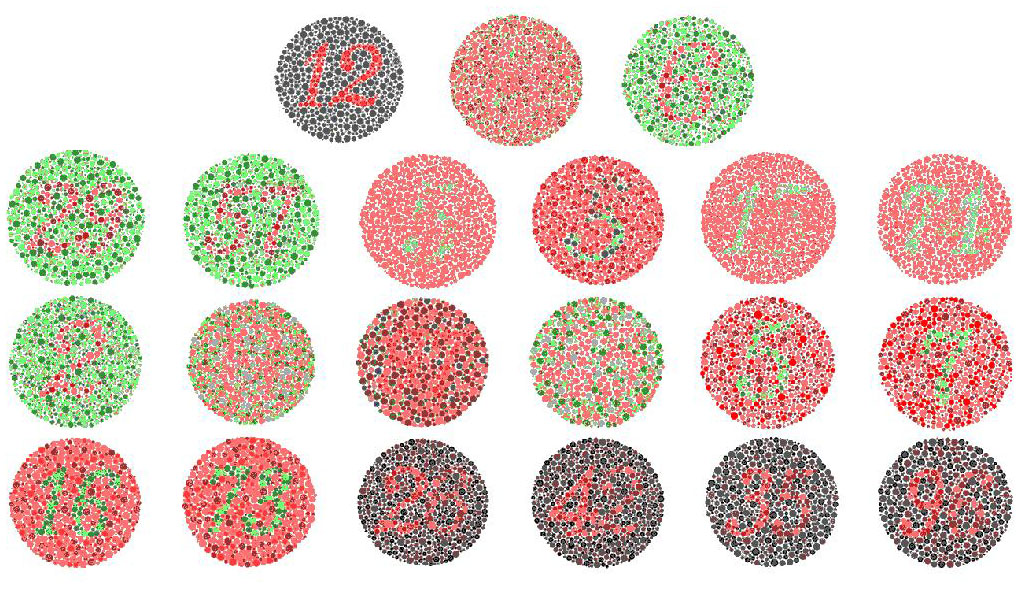
\includegraphics[width=0.90\textwidth]{figuraDeslocarHSeI.jpg}
\caption{Resultado da aplicação das Equações \ref{eq:reduzirHpara3}, \ref{eq:reduzirS} e \ref{eq:reduzirI} sobre a Figura \ref{fig:platesIshihara}. \label{fig:reduzirHSeI}}
\end{figure}

Os resultados apresentados nesta Subseção não foram satisfatórios. Para poucas pranchas contidas na Figura \ref{fig:platesIshihara}, o número contido dentro dessas pranchas ficou mais fácil de ser identificado após os processamentos descritos. 

Foram implementados outros dois processamentos com o objetivo de deslocar os valores da matiz, um resumo de cada um desses processamentos encontra-se abaixo:

\begin{enumerate}
\item \textbf{Distanciar os valores próximos a $60^o$:} O valor que representa o valor de amarelo em H é $60^o$. Amarelo está exatamente entre o verde e o vermelho. A maioria dos daltônicos possuem dificuldade para distinguir verde e vermelho, conforme descrito na Seção \ref{sec:tiposDaltonismo}. Por esses motivos entende-se que as cores que a maioria dos daltônicos possuem dificuldade de enxergar estão entre o vermelho e o verde. Afim de distanciar essas cores, os valores do intervalo $[0^o;60^o]$ foram compactados no intervalo $[320^o;360^o$] e todos os valores do intervalo $[240^o;360^o]$ foram compactados no intervalo $[240^o;320^o[$. Analogamente, os valores do intervalo $]60^o;120^o]$ foram compactados no intervalo $[120^o; 160^o]$ e todos os valores do intervalo $[120^o;240^o[$ foram compactados no intervalo $]160^o;240^o[$. A Figura \ref{fig:reduzirHamarelo} ilustra esse processamento sobre a Figura sobre a Figura \ref{fig:platesIshihara}.
\end{enumerate}


Um deles distanciava os valores próximos a $60^o$, pois o amarelo está entre o verde e o vermelho, cores que a maioria dos daltônicos possuem dificuldade de distingur.

As equações apresentadas limitam as cores, tornando-as mais fácil de identificar as diferenças entre as cores pela maioria dos daltônicos. No entanto, devido a impactante abstração dos sistemas de cores HSV e HSI, muitas características as quais os daltônicos não conseguiam identificar antes do processamento são perdidas, tornando assim a identificação dessas características impossível em alguns casos.


\subsection{Elevar os valores da intensidade ou valor}
\label{subsec:deslocarVouI}

Assim como o processamento apresentado na Subseção \ref{subsec:deslocarH}, esse processamento é iniciado com a conversão de uma imagem RGB para o sistema de cores HSV ou HSI, após essa conversão outro processamento é realizado no sistema de cores HSV ou HSI e por fim a imagem é convertida de volta para o sistema de cores RGB. As conversão entre os sistemas de cores não são descritas nos processamentos apresentados, entende-se que elas são obrigatórias para todos os processamentos descritos neste trabalho.

A ideia básica desse processamento é simples, ela consiste em multiplicar os valores de V ou I por um escalar. Quanto maior esse escalar, mais vibrante ou intensa a cor. Porém, é necessário verificar se o resultado dessa multiplicação não é maior do que o maior valor permitido para os elementos de V ou I, ou seja, se não é maior do que $1$. Para o sistema de cores HSV, esse processamento é descrito na Equação \ref{eq:elevarV} e para o sistema de cores HSI, na Equação \ref{eq:elevarI}.

\begin{equation}
\label{eq:elevarV}
V'=\left\{
\begin{array}{rc}
       3 \times V,&\mbox{se}\quad 3 \times V < 1 \\
       1,&\mbox{caso contrário}
\end{array}\right.
\end{equation}

\begin{equation}
\label{eq:elevarI}
I'=\left\{
\begin{array}{rc}
       3 \times I,&\mbox{se}\quad 3 \times I < 1 \\
       1,&\mbox{caso contrário}
\end{array}\right.
\end{equation}



\subsection{Sistema HSV}
\label{subsec:alterarValues} 

\subsection{Sistema HSI}

O sistema de cores HSI é semelhante ao sistema de cores HSV, por isso todos os processamentos realizados no sistema de cores HSV podem ser facilmente modificados para o sistema HSI.

Sendo assim, foram modificados os algoritmos desenvolvidos para o sistema de cores HSV e abaixo podemos ver o resultado para algumas pranchas de Ishihara.

Inserir imagens

Inserir imagens

Inserir imagens

Inserir imagens

Inserir imagens

Inserir imagens

Comparar o resultado do processamento de imagem entre os sistemas de cores HSI e HSV.

\subsection{Sistema LMS}


\section{Ferramenta}

Para obter resultados das pessoas daltônicas, foi criado um site utilizando a plataforma \citeonline{googleappengine2015}. Essa plataforma utiliza o conceito de nuvem e é classificada como PaaS (Plataforma como um serviço, do inglês Platform as a Service). É possível utilizar as linguagens de programação Python, Java, PHP ou GO para desenvolver aplicativos que serão hospedados no Google App Engine. Devido a experiência do proponente com a linguagem de programação Java, essa foi a linguagem de programação escolhida para o desenvolvimento do site. 

Para salvar as informações geradas através do uso da aplicação por usuários, foi utilizado o banco de dados do Google App Engine. Esse banco de dados utiliza o conceito NoSQL. Afim de facilitar a programação para acesso, alteração e armazenamento nesse banco de dados, foi utilizada a API (Interface de Programação de Aplicativos, do inglês Application Programming Interface) para acesso de dados chamada \citeonline{objectify2015}.

Para facilitar a criação do layout da aplicação, foi utilizado o framework \citeonline{Bootstrap}. Com esse framework, é possível criar a interface com o usuário mais rápido e mais facilmente do que sem ele.

A ferramenda possui quatro telas principais, são elas:

\begin{itemize}
\item Teste original;
\item Teste modificado;
\item Pesquisa;
\item Sobre.
\end{itemize}

Abaixo são apresentados detalhes de cada uma dessas telas.

\subsection{Teste original}
O teste original utiliza as 21 pranchas de Ishihara que estão na Figura \ref{fig:figuraTesteOriginalFerramenta}. Nesse teste, o usuário deve digitar o número visto em cada uma das imagens e no final é apresentado o resultado do teste. 

Foi percebido que o contraste do dispositivo utilizado para a realização do teste influencia no resultado. Por esse e por outros motivos, não é possível definir se uma pessoa é daltônica somente após a realização do teste de Ishihara. No entanto, juntamente com o resultado do teste, é apresentado ao usuário se com base no resultado do teste ele possui indício de ser daltônico. Também é apresentada uma mensagem ao usuário recomendando a procura de um especialista para um diagnóstico preciso.

\begin{figure}[!htb]
\centering 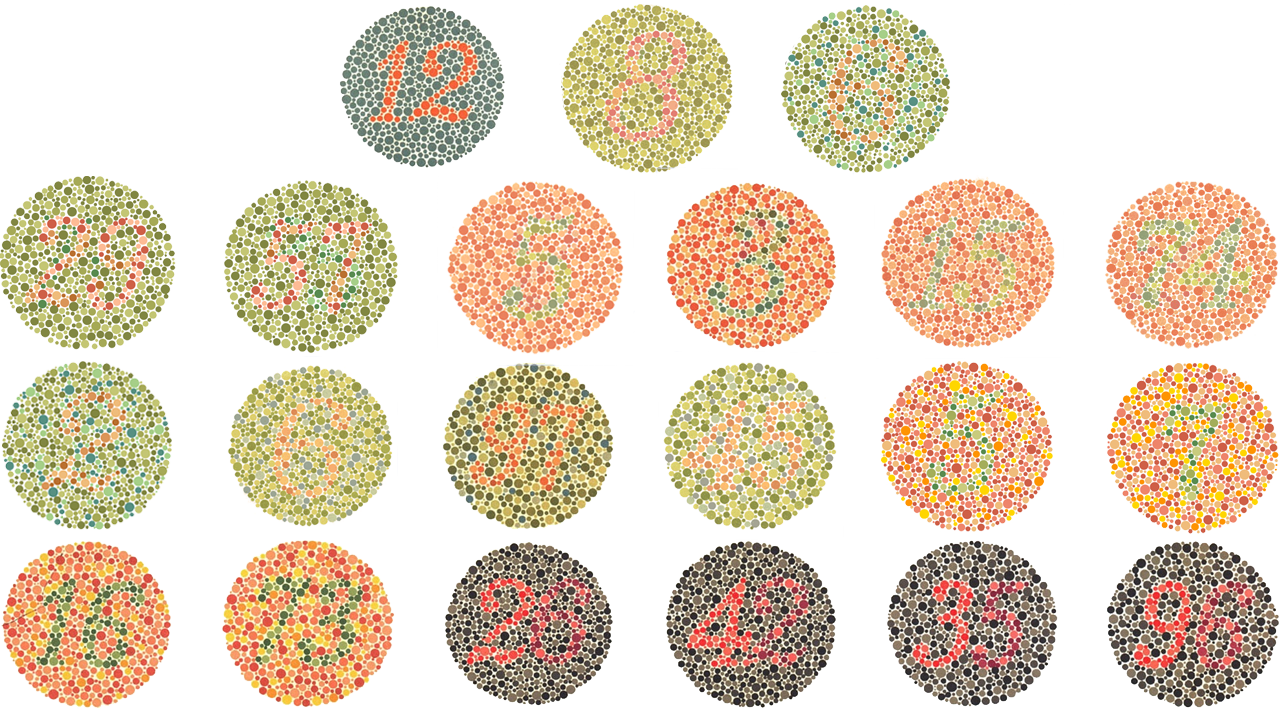
\includegraphics[width=0.9\textwidth]{platesIshihara.png}
\caption{Pranchas utilizadas no teste de Ishihara da Ferramenta. (adaptado de \citeonline{colorblindnesssite})} \label{fig:figuraTesteOriginalFerramenta}
\end{figure}


\subsection{Teste modificado}

Essa página é composta pelo teste de Ishihara com as suas imagens modificadas. As modificações foram feitas conforme o processamento de imagens descrito na Subseção \ref{subsec:alterarValues}, a qual utiliza o sistema de cores HSV.

Os parâmetros para o algoritmo desenvolvido para a realização desse processamento são controlados através de barras de controle e caixas de seleção, conforme é possível visualizar na Figura \ref{fig:figuraParametrosTeste}.

As caixas de seleção Verde, Vermelho e azul.................................................. .................................................. .................................................. .................................................. .................................................. ..................................................

A barra de controle cores..................................................
..................................................
..................................................
0 significa XXXXXXX, 1 significa YYYYYYY, 2 significa QQQQQQQQQ,
3 significa XXXXXXX, 4 significa YYYYYYY, 5 significa QQQQQQQQQ,

A barra de controle saturação..................................................
..................................................
..................................................
0 significa XXXXXXX, 1 significa YYYYYYY, 2 significa QQQQQQQQQ,
3 significa XXXXXXX, 4 significa YYYYYYY, 5 significa QQQQQQQQQ,

A barra de controle intensidade..................................................
..................................................
..................................................
0 significa XXXXXXX, 1 significa YYYYYYY, 2 significa QQQQQQQQQ,
3 significa XXXXXXX, 4 significa YYYYYYY, 5 significa QQQQQQQQQ,

\begin{figure}[!htb]
\centering 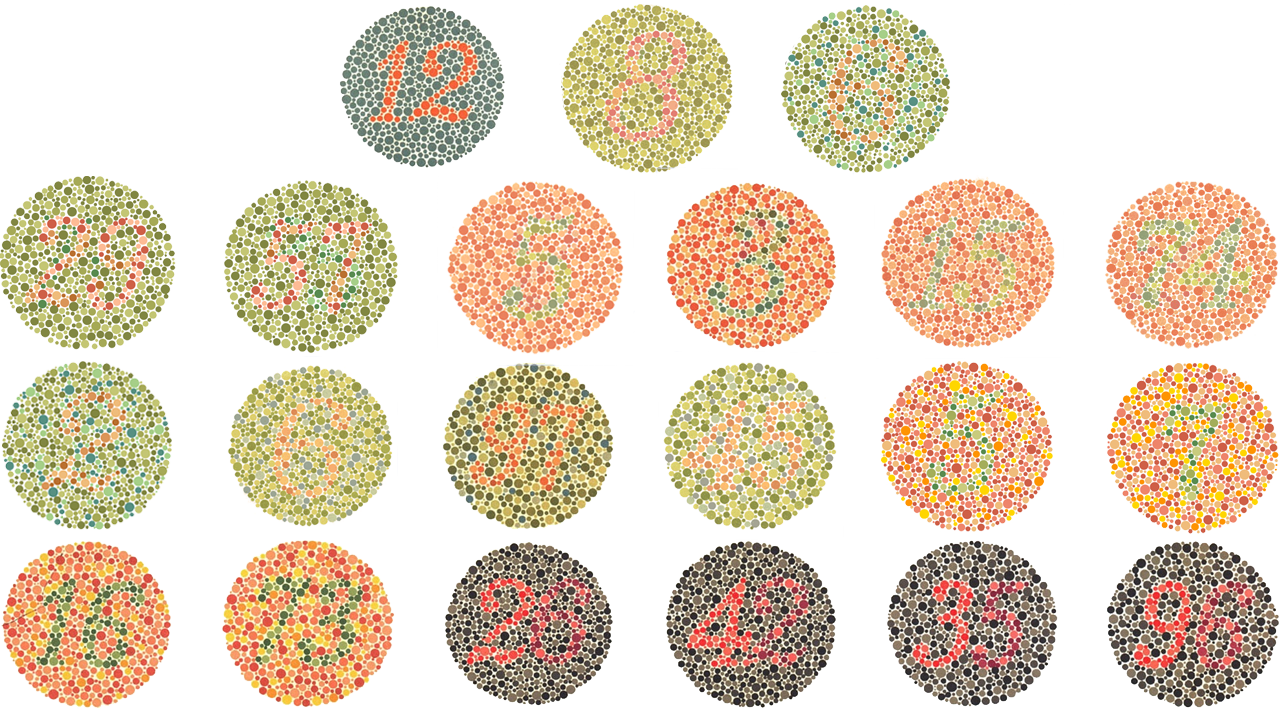
\includegraphics[width=0.6\textwidth]{platesIshihara.png}
\caption{Alterar imagem} \label{fig:figuraParametrosTeste}
\end{figure}

\subsection{Pesquisa}

Essa página é composta por um formulário que foi utilizado para obter informações adicionais dos usuários, com o objetivo de fortalecer os argumentos da conclusão sobre a ferramenta. Quando um usuário responde o formulário, as respostas vão para o banco de dados do Google App Engine, atreladas ao e-mail do usuário que respondeu as perguntas.


As perguntas contidas nesse formulário são....

1

2

3

4

5

6

7

8

9

\subsection{Sobre}

Nenhum ação do usuário é esperada nessa tela. Ela possui o objetivo de informar ao usuário qual o objetivo deste trabalho e quem são as pessoas que estão envolvidas no seu desenvolvimento.

É possível visualizar as informações apresentadas nessa tela na Figura \ref{fig:figuraSobre}.

\begin{figure}[!htb]
\centering 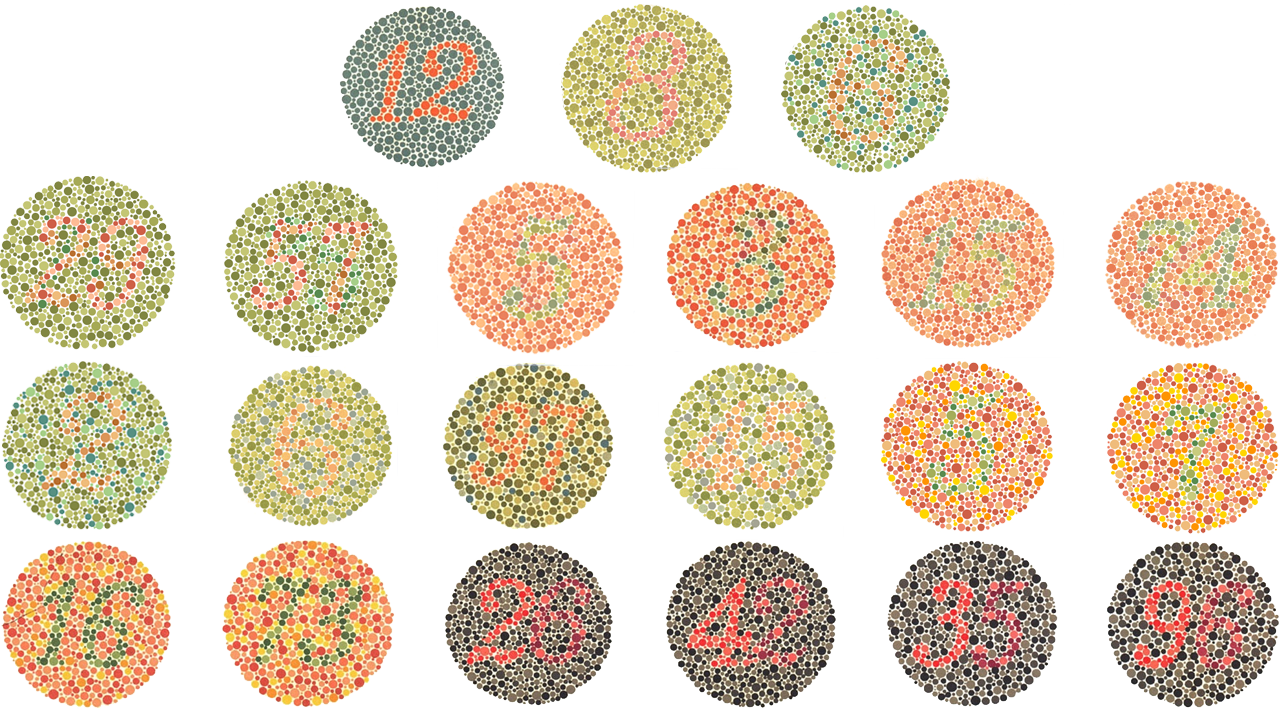
\includegraphics[width=0.6\textwidth]{platesIshihara.png}
\caption{Alterar imagem} \label{fig:figuraSobre}
\end{figure}

% ---
% Conclusão
% ---
\chapter{Conclusão}
% ----------------------------------------------------------
% ELEMENTOS PÓS-TEXTUAIS
% ----------------------------------------------------------
\postextual


% ----------------------------------------------------------
% Referências bibliográficas
% ----------------------------------------------------------
%\bibliographystyle{plain}
\bibliography{references}

% ----------------------------------------------------------
% Glossário
% ----------------------------------------------------------
%
% Consulte o manual da classe abntex2 para orientações sobre o glossário.
%
%\glossary

% ----------------------------------------------------------
% Apêndices
% ----------------------------------------------------------

% ---
% Inicia os apêndices
% ---
\begin{apendicesenv}

% Imprime uma página indicando o início dos apêndices
\partapendices

% ----------------------------------------------------------
\chapter{Imagens do teste de Ishihara}
% ----------------------------------------------------------
\label{ap:ishihara}

Esse apêndice contém pranchas do teste de Ishihara. Essas pranchas estão separadas em tipos, conforme definido na Subseção \ref{subsection:Ishihara}. Além disso, na Figura \ref{fig:apendiceExample} são apresentadas duas pranchas de demonstração, onde as pessoas daltônicas e as não daltônicas visualizam o mesmo conteúdo dentro dessas pranchas. Nessa imagem, todas as pessoas devem visualizar o número 12 na imagem (a) e uma linha na imagem (b).

\begin{figure}[!htb]
\minipage{0.40\textwidth}
\centering
{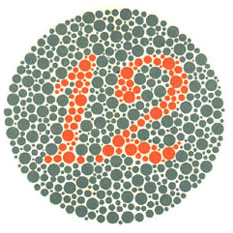
\includegraphics[width=\linewidth]{ishihara-exemplos/plate1.jpg}}
(a)
\endminipage\hfill
\minipage{0.40\textwidth}
\centering
{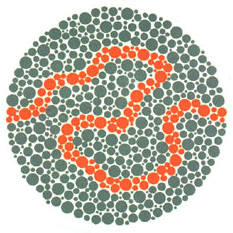
\includegraphics[width=\linewidth]{ishihara-exemplos/plate38.jpg}}
(b)
\endminipage\hfill
\caption{Pranchas de demonstração do teste de Ishihara. (retirado de \citeonline{colorblindnesssite})}
\label{fig:apendiceExample}
\end{figure}

Nas pranchas da Figura \ref{fig:apendiceDigitoEscondido}, apenas daltônicos conseguem visualizar os números. Os daltônicos visualizam o número 5 em (a), o número 2 em (b), o número 45 em (c) e o número 73 em (d).

Na Figura \ref{fig:apendiceFuga},  apenas pessoas não daltônicas conseguem visualizar o número ou as linhas nas pranchas. Na imagem (a) está o número 2, em (b) o número 6, em (c) o número 97, em (d) o número 45, em (e) o número 5, em (f) o número 7, em (g) o número 16, em (h) o número 73 e nas imagens (i), (j), (k), (l), (m), (n), (o) e (p) uma linha é visível as pessoas não daltônicas.

Nas pranchas da Figura \ref{fig:apendiceTransformacao}, pessoas daltônicas visualizam algo diferente do que é visto por pessoas não daltônicas. Na imagem (a) daltônicos visualizam o número 3 e pessoas com visão normal o número 8, em (b) daltônicos visualizam 2 e outras pessoas 5, em (c) daltônicos visualizam 5 e outras pessoas 3, em (d) daltônicos visualizam 17 e outras pessoas 15, em (e) daltônicos visualizam 21 e outras pessoas 74, em (f) daltônicos visualizam 5 e outras pessoas 6, em (g) daltônicos visualizam 70 e outras pessoas 29 e em (h) daltônicos visualizam 35 e outras pessoas 57.

Na Figura \ref{fig:apendiceClassificacao}, o objetivo das pranchas é diferenciar os daltônicos que possuem deficiência nos cones do tipo M (que capturam o verde) e os daltônicos que possuem deficiência nos cones do tipo L (que capturam o vermelho). Na imagem (a) pessoas não daltônicas visualizam 26, daltônicos com deficiência nos cones do tipo M visualizam o 2 e o número 6 embaçado e daltônicos com deficiência nos cones do tipo L visualizam o 6 e o número 2 embaçado. Na imagem (b) pessoas não daltônicas visualizam 42, daltônicos com deficiência nos cones do tipo M visualizam o 4 e o número 2 embaçado e daltônicos com deficiência nos cones do tipo L visualizam o 2 e o número 4 embaçado. Na imagem (c) pessoas não daltônicas visualizam 35, daltônicos com deficiência nos cones do tipo M visualizam o 3 e o número 5 embaçado e daltônicos com deficiência nos cones do tipo L visualizam o 5 e o número 3 embaçado. Na imagem (d) pessoas não daltônicas visualizam 96, daltônicos com deficiência nos cones do tipo M visualizam o 9 e o número 6 embaçado e daltônicos com deficiência nos cones do tipo L visualizam o 6 e o número 9 embaçado. 

\begin{figure}[!htb]
\minipage{0.40\textwidth}
\centering
{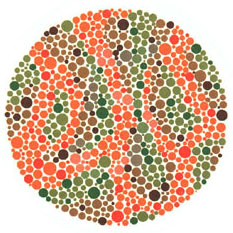
\includegraphics[width=\linewidth]{ishihara-digitoescondido/plate18.jpg}}
(a)
\endminipage\hfill
\minipage{0.40\textwidth}
\centering
{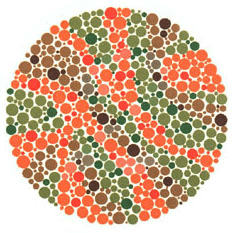
\includegraphics[width=\linewidth]{ishihara-digitoescondido/plate19.jpg}}
(b)
\endminipage\hfill

\minipage{0.40\textwidth}
\centering
{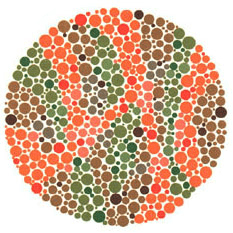
\includegraphics[width=\linewidth]{ishihara-digitoescondido/plate20.jpg}}
(c)
\endminipage\hfill
\minipage{0.40\textwidth}
\centering
{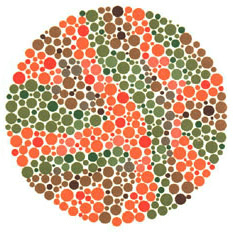
\includegraphics[width=\linewidth]{ishihara-digitoescondido/plate21.jpg}}
(d)
\endminipage\hfill
\caption{Imagens do teste de Ishihara do tipo dígito escondido. (adaptado de \citeonline{colorblindnesssite})}
\label{fig:apendiceDigitoEscondido}
\end{figure}

\begin{figure}[!htb]
\minipage{0.22\textwidth}
\centering
{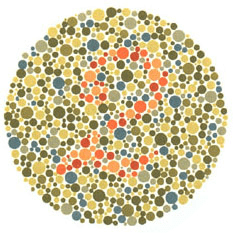
\includegraphics[width=\linewidth]{ishihara-fuga/plate10.jpg}}
(a)
\endminipage\hfill
\minipage{0.22\textwidth}
\centering
{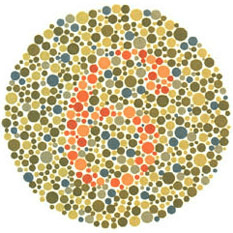
\includegraphics[width=\linewidth]{ishihara-fuga/plate11.jpg}}
(b)
\endminipage\hfill
\minipage{0.22\textwidth}
\centering
{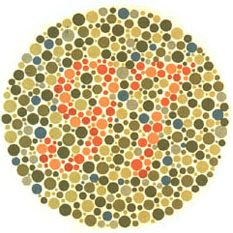
\includegraphics[width=\linewidth]{ishihara-fuga/plate12.jpg}}
(c)
\endminipage\hfill
\minipage{0.22\textwidth}
\centering
{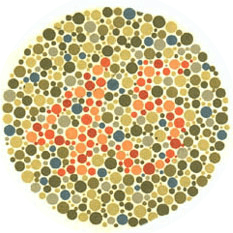
\includegraphics[width=\linewidth]{ishihara-fuga/plate13.jpg}}
(d)
\endminipage\hfill

\minipage{0.22\textwidth}
\centering
{\includegraphics[width=\linewidth]{ishihara-fuga/plate14.jpg}}
(e)
\endminipage\hfill
\minipage{0.22\textwidth}
\centering
{\includegraphics[width=\linewidth]{ishihara-fuga/plate15.jpg}}
(f)
\endminipage\hfill
\minipage{0.22\textwidth}
\centering
{\includegraphics[width=\linewidth]{ishihara-fuga/plate16.jpg}}
(g)
\endminipage\hfill
\minipage{0.22\textwidth}
\centering
{\includegraphics[width=\linewidth]{ishihara-fuga/plate17.jpg}}
(h)
\endminipage\hfill

\minipage{0.22\textwidth}
\centering
{\includegraphics[width=\linewidth]{ishihara-fuga/plate30.jpg}}
(i)
\endminipage\hfill
\minipage{0.22\textwidth}
\centering
{\includegraphics[width=\linewidth]{ishihara-fuga/plate31.jpg}}
(j)
\endminipage\hfill
\minipage{0.22\textwidth}
\centering
{\includegraphics[width=\linewidth]{ishihara-fuga/plate32.jpg}}
(k)
\endminipage\hfill
\minipage{0.22\textwidth}
\centering
{\includegraphics[width=\linewidth]{ishihara-fuga/plate33.jpg}}
(l)

\endminipage\hfill
\minipage{0.22\textwidth}
\centering
{\includegraphics[width=\linewidth]{ishihara-fuga/plate34.jpg}}
(m)
\endminipage\hfill
\minipage{0.22\textwidth}
\centering
{\includegraphics[width=\linewidth]{ishihara-fuga/plate35.jpg}}
(n)
\endminipage\hfill
\minipage{0.22\textwidth}
\centering
{\includegraphics[width=\linewidth]{ishihara-fuga/plate36.jpg}}
(o)
\endminipage\hfill
\minipage{0.22\textwidth}
\centering
{\includegraphics[width=\linewidth]{ishihara-fuga/plate37.jpg}}
(p)
\endminipage\hfill


\caption{Imagens do teste de Ishihara do tipo fuga. (adaptado de \citeonline{colorblindnesssite})}
\label{fig:apendiceFuga}

\end{figure}



\begin{figure}[!htb]
\minipage{0.29\textwidth}
\centering
{\includegraphics[width=\linewidth]{ishihara-transformacao/plate2.jpg}}
(a)
\endminipage\hfill
\minipage{0.29\textwidth}
\centering
{\includegraphics[width=\linewidth]{ishihara-transformacao/plate6.jpg}}
(b)
\endminipage\hfill
\minipage{0.29\textwidth}
\centering
{\includegraphics[width=\linewidth]{ishihara-transformacao/plate7.jpg}}
(c)
\endminipage\hfill

\minipage{0.29\textwidth}
\centering
{\includegraphics[width=\linewidth]{ishihara-transformacao/plate8.jpg}}
(d)
\endminipage\hfill
\minipage{0.29\textwidth}
\centering
{\includegraphics[width=\linewidth]{ishihara-transformacao/plate9.jpg}}
(e)
\endminipage\hfill
\minipage{0.29\textwidth}
\centering
{\includegraphics[width=\linewidth]{ishihara-transformacao/plate3.jpg}}
(f)
\endminipage\hfill

\minipage{0.29\textwidth}
\centering
{\includegraphics[width=\linewidth]{ishihara-transformacao/plate4.jpg}}
(g)
\endminipage\hfill
\minipage{0.29\textwidth}
\centering
{\includegraphics[width=\linewidth]{ishihara-transformacao/plate5.jpg}}
(h)
\endminipage\hfill


\caption{Imagens do teste de Ishihara do tipo transfomação. (adaptado de \citeonline{colorblindnesssite})}
\label{fig:apendiceTransformacao}

\end{figure}

\begin{figure}[!htb]
\minipage{0.40\textwidth}
\centering
{\includegraphics[width=\linewidth]{ishihara-classificacao/plate22.jpg}}
(a)
\endminipage\hfill
\minipage{0.40\textwidth}
\centering
{\includegraphics[width=\linewidth]{ishihara-classificacao/plate23.jpg}}
(b)
\endminipage\hfill


\minipage{0.40\textwidth}
\centering
{\includegraphics[width=\linewidth]{ishihara-classificacao/plate24.jpg}}
(c)
\endminipage\hfill
\minipage{0.40\textwidth}
\centering
{\includegraphics[width=\linewidth]{ishihara-classificacao/plate25.jpg}}
(d)
\endminipage\hfill

\caption{Imagens do teste de Ishihara do tipo classificação. (adaptado de \citeonline{colorblindnesssite})}
\label{fig:apendiceClassificacao}

\end{figure}


\end{apendicesenv}
% ---

\end{document}